
% Default to the notebook output style

    


% Inherit from the specified cell style.




    
\documentclass[11pt]{article}

    
    
    \usepackage[T1]{fontenc}
    % Nicer default font (+ math font) than Computer Modern for most use cases
    \usepackage{mathpazo}

    % Basic figure setup, for now with no caption control since it's done
    % automatically by Pandoc (which extracts ![](path) syntax from Markdown).
    \usepackage{graphicx}
    % We will generate all images so they have a width \maxwidth. This means
    % that they will get their normal width if they fit onto the page, but
    % are scaled down if they would overflow the margins.
    \makeatletter
    \def\maxwidth{\ifdim\Gin@nat@width>\linewidth\linewidth
    \else\Gin@nat@width\fi}
    \makeatother
    \let\Oldincludegraphics\includegraphics
    % Set max figure width to be 80% of text width, for now hardcoded.
    \renewcommand{\includegraphics}[1]{\Oldincludegraphics[width=.8\maxwidth]{#1}}
    % Ensure that by default, figures have no caption (until we provide a
    % proper Figure object with a Caption API and a way to capture that
    % in the conversion process - todo).
    \usepackage{caption}
    \DeclareCaptionLabelFormat{nolabel}{}
    \captionsetup{labelformat=nolabel}

    \usepackage{adjustbox} % Used to constrain images to a maximum size 
    \usepackage{xcolor} % Allow colors to be defined
    \usepackage{enumerate} % Needed for markdown enumerations to work
    \usepackage{geometry} % Used to adjust the document margins
    \usepackage{amsmath} % Equations
    \usepackage{amssymb} % Equations
    \usepackage{textcomp} % defines textquotesingle
    % Hack from http://tex.stackexchange.com/a/47451/13684:
    \AtBeginDocument{%
        \def\PYZsq{\textquotesingle}% Upright quotes in Pygmentized code
    }
    \usepackage{upquote} % Upright quotes for verbatim code
    \usepackage{eurosym} % defines \euro
    \usepackage[mathletters]{ucs} % Extended unicode (utf-8) support
    \usepackage[utf8x]{inputenc} % Allow utf-8 characters in the tex document
    \usepackage{fancyvrb} % verbatim replacement that allows latex
    \usepackage{grffile} % extends the file name processing of package graphics 
                         % to support a larger range 
    % The hyperref package gives us a pdf with properly built
    % internal navigation ('pdf bookmarks' for the table of contents,
    % internal cross-reference links, web links for URLs, etc.)
    \usepackage{hyperref}
    \usepackage{longtable} % longtable support required by pandoc >1.10
    \usepackage{booktabs}  % table support for pandoc > 1.12.2
    \usepackage[inline]{enumitem} % IRkernel/repr support (it uses the enumerate* environment)
    \usepackage[normalem]{ulem} % ulem is needed to support strikethroughs (\sout)
                                % normalem makes italics be italics, not underlines
    

    
    
    % Colors for the hyperref package
    \definecolor{urlcolor}{rgb}{0,.145,.698}
    \definecolor{linkcolor}{rgb}{.71,0.21,0.01}
    \definecolor{citecolor}{rgb}{.12,.54,.11}

    % ANSI colors
    \definecolor{ansi-black}{HTML}{3E424D}
    \definecolor{ansi-black-intense}{HTML}{282C36}
    \definecolor{ansi-red}{HTML}{E75C58}
    \definecolor{ansi-red-intense}{HTML}{B22B31}
    \definecolor{ansi-green}{HTML}{00A250}
    \definecolor{ansi-green-intense}{HTML}{007427}
    \definecolor{ansi-yellow}{HTML}{DDB62B}
    \definecolor{ansi-yellow-intense}{HTML}{B27D12}
    \definecolor{ansi-blue}{HTML}{208FFB}
    \definecolor{ansi-blue-intense}{HTML}{0065CA}
    \definecolor{ansi-magenta}{HTML}{D160C4}
    \definecolor{ansi-magenta-intense}{HTML}{A03196}
    \definecolor{ansi-cyan}{HTML}{60C6C8}
    \definecolor{ansi-cyan-intense}{HTML}{258F8F}
    \definecolor{ansi-white}{HTML}{C5C1B4}
    \definecolor{ansi-white-intense}{HTML}{A1A6B2}

    % commands and environments needed by pandoc snippets
    % extracted from the output of `pandoc -s`
    \providecommand{\tightlist}{%
      \setlength{\itemsep}{0pt}\setlength{\parskip}{0pt}}
    \DefineVerbatimEnvironment{Highlighting}{Verbatim}{commandchars=\\\{\}}
    % Add ',fontsize=\small' for more characters per line
    \newenvironment{Shaded}{}{}
    \newcommand{\KeywordTok}[1]{\textcolor[rgb]{0.00,0.44,0.13}{\textbf{{#1}}}}
    \newcommand{\DataTypeTok}[1]{\textcolor[rgb]{0.56,0.13,0.00}{{#1}}}
    \newcommand{\DecValTok}[1]{\textcolor[rgb]{0.25,0.63,0.44}{{#1}}}
    \newcommand{\BaseNTok}[1]{\textcolor[rgb]{0.25,0.63,0.44}{{#1}}}
    \newcommand{\FloatTok}[1]{\textcolor[rgb]{0.25,0.63,0.44}{{#1}}}
    \newcommand{\CharTok}[1]{\textcolor[rgb]{0.25,0.44,0.63}{{#1}}}
    \newcommand{\StringTok}[1]{\textcolor[rgb]{0.25,0.44,0.63}{{#1}}}
    \newcommand{\CommentTok}[1]{\textcolor[rgb]{0.38,0.63,0.69}{\textit{{#1}}}}
    \newcommand{\OtherTok}[1]{\textcolor[rgb]{0.00,0.44,0.13}{{#1}}}
    \newcommand{\AlertTok}[1]{\textcolor[rgb]{1.00,0.00,0.00}{\textbf{{#1}}}}
    \newcommand{\FunctionTok}[1]{\textcolor[rgb]{0.02,0.16,0.49}{{#1}}}
    \newcommand{\RegionMarkerTok}[1]{{#1}}
    \newcommand{\ErrorTok}[1]{\textcolor[rgb]{1.00,0.00,0.00}{\textbf{{#1}}}}
    \newcommand{\NormalTok}[1]{{#1}}
    
    % Additional commands for more recent versions of Pandoc
    \newcommand{\ConstantTok}[1]{\textcolor[rgb]{0.53,0.00,0.00}{{#1}}}
    \newcommand{\SpecialCharTok}[1]{\textcolor[rgb]{0.25,0.44,0.63}{{#1}}}
    \newcommand{\VerbatimStringTok}[1]{\textcolor[rgb]{0.25,0.44,0.63}{{#1}}}
    \newcommand{\SpecialStringTok}[1]{\textcolor[rgb]{0.73,0.40,0.53}{{#1}}}
    \newcommand{\ImportTok}[1]{{#1}}
    \newcommand{\DocumentationTok}[1]{\textcolor[rgb]{0.73,0.13,0.13}{\textit{{#1}}}}
    \newcommand{\AnnotationTok}[1]{\textcolor[rgb]{0.38,0.63,0.69}{\textbf{\textit{{#1}}}}}
    \newcommand{\CommentVarTok}[1]{\textcolor[rgb]{0.38,0.63,0.69}{\textbf{\textit{{#1}}}}}
    \newcommand{\VariableTok}[1]{\textcolor[rgb]{0.10,0.09,0.49}{{#1}}}
    \newcommand{\ControlFlowTok}[1]{\textcolor[rgb]{0.00,0.44,0.13}{\textbf{{#1}}}}
    \newcommand{\OperatorTok}[1]{\textcolor[rgb]{0.40,0.40,0.40}{{#1}}}
    \newcommand{\BuiltInTok}[1]{{#1}}
    \newcommand{\ExtensionTok}[1]{{#1}}
    \newcommand{\PreprocessorTok}[1]{\textcolor[rgb]{0.74,0.48,0.00}{{#1}}}
    \newcommand{\AttributeTok}[1]{\textcolor[rgb]{0.49,0.56,0.16}{{#1}}}
    \newcommand{\InformationTok}[1]{\textcolor[rgb]{0.38,0.63,0.69}{\textbf{\textit{{#1}}}}}
    \newcommand{\WarningTok}[1]{\textcolor[rgb]{0.38,0.63,0.69}{\textbf{\textit{{#1}}}}}
    
    
    % Define a nice break command that doesn't care if a line doesn't already
    % exist.
    \def\br{\hspace*{\fill} \\* }
    % Math Jax compatability definitions
    \def\gt{>}
    \def\lt{<}
    % Document parameters
    \title{Cross-correlation, Convolutional}
    
    
    

    % Pygments definitions
    
\makeatletter
\def\PY@reset{\let\PY@it=\relax \let\PY@bf=\relax%
    \let\PY@ul=\relax \let\PY@tc=\relax%
    \let\PY@bc=\relax \let\PY@ff=\relax}
\def\PY@tok#1{\csname PY@tok@#1\endcsname}
\def\PY@toks#1+{\ifx\relax#1\empty\else%
    \PY@tok{#1}\expandafter\PY@toks\fi}
\def\PY@do#1{\PY@bc{\PY@tc{\PY@ul{%
    \PY@it{\PY@bf{\PY@ff{#1}}}}}}}
\def\PY#1#2{\PY@reset\PY@toks#1+\relax+\PY@do{#2}}

\expandafter\def\csname PY@tok@w\endcsname{\def\PY@tc##1{\textcolor[rgb]{0.73,0.73,0.73}{##1}}}
\expandafter\def\csname PY@tok@c\endcsname{\let\PY@it=\textit\def\PY@tc##1{\textcolor[rgb]{0.25,0.50,0.50}{##1}}}
\expandafter\def\csname PY@tok@cp\endcsname{\def\PY@tc##1{\textcolor[rgb]{0.74,0.48,0.00}{##1}}}
\expandafter\def\csname PY@tok@k\endcsname{\let\PY@bf=\textbf\def\PY@tc##1{\textcolor[rgb]{0.00,0.50,0.00}{##1}}}
\expandafter\def\csname PY@tok@kp\endcsname{\def\PY@tc##1{\textcolor[rgb]{0.00,0.50,0.00}{##1}}}
\expandafter\def\csname PY@tok@kt\endcsname{\def\PY@tc##1{\textcolor[rgb]{0.69,0.00,0.25}{##1}}}
\expandafter\def\csname PY@tok@o\endcsname{\def\PY@tc##1{\textcolor[rgb]{0.40,0.40,0.40}{##1}}}
\expandafter\def\csname PY@tok@ow\endcsname{\let\PY@bf=\textbf\def\PY@tc##1{\textcolor[rgb]{0.67,0.13,1.00}{##1}}}
\expandafter\def\csname PY@tok@nb\endcsname{\def\PY@tc##1{\textcolor[rgb]{0.00,0.50,0.00}{##1}}}
\expandafter\def\csname PY@tok@nf\endcsname{\def\PY@tc##1{\textcolor[rgb]{0.00,0.00,1.00}{##1}}}
\expandafter\def\csname PY@tok@nc\endcsname{\let\PY@bf=\textbf\def\PY@tc##1{\textcolor[rgb]{0.00,0.00,1.00}{##1}}}
\expandafter\def\csname PY@tok@nn\endcsname{\let\PY@bf=\textbf\def\PY@tc##1{\textcolor[rgb]{0.00,0.00,1.00}{##1}}}
\expandafter\def\csname PY@tok@ne\endcsname{\let\PY@bf=\textbf\def\PY@tc##1{\textcolor[rgb]{0.82,0.25,0.23}{##1}}}
\expandafter\def\csname PY@tok@nv\endcsname{\def\PY@tc##1{\textcolor[rgb]{0.10,0.09,0.49}{##1}}}
\expandafter\def\csname PY@tok@no\endcsname{\def\PY@tc##1{\textcolor[rgb]{0.53,0.00,0.00}{##1}}}
\expandafter\def\csname PY@tok@nl\endcsname{\def\PY@tc##1{\textcolor[rgb]{0.63,0.63,0.00}{##1}}}
\expandafter\def\csname PY@tok@ni\endcsname{\let\PY@bf=\textbf\def\PY@tc##1{\textcolor[rgb]{0.60,0.60,0.60}{##1}}}
\expandafter\def\csname PY@tok@na\endcsname{\def\PY@tc##1{\textcolor[rgb]{0.49,0.56,0.16}{##1}}}
\expandafter\def\csname PY@tok@nt\endcsname{\let\PY@bf=\textbf\def\PY@tc##1{\textcolor[rgb]{0.00,0.50,0.00}{##1}}}
\expandafter\def\csname PY@tok@nd\endcsname{\def\PY@tc##1{\textcolor[rgb]{0.67,0.13,1.00}{##1}}}
\expandafter\def\csname PY@tok@s\endcsname{\def\PY@tc##1{\textcolor[rgb]{0.73,0.13,0.13}{##1}}}
\expandafter\def\csname PY@tok@sd\endcsname{\let\PY@it=\textit\def\PY@tc##1{\textcolor[rgb]{0.73,0.13,0.13}{##1}}}
\expandafter\def\csname PY@tok@si\endcsname{\let\PY@bf=\textbf\def\PY@tc##1{\textcolor[rgb]{0.73,0.40,0.53}{##1}}}
\expandafter\def\csname PY@tok@se\endcsname{\let\PY@bf=\textbf\def\PY@tc##1{\textcolor[rgb]{0.73,0.40,0.13}{##1}}}
\expandafter\def\csname PY@tok@sr\endcsname{\def\PY@tc##1{\textcolor[rgb]{0.73,0.40,0.53}{##1}}}
\expandafter\def\csname PY@tok@ss\endcsname{\def\PY@tc##1{\textcolor[rgb]{0.10,0.09,0.49}{##1}}}
\expandafter\def\csname PY@tok@sx\endcsname{\def\PY@tc##1{\textcolor[rgb]{0.00,0.50,0.00}{##1}}}
\expandafter\def\csname PY@tok@m\endcsname{\def\PY@tc##1{\textcolor[rgb]{0.40,0.40,0.40}{##1}}}
\expandafter\def\csname PY@tok@gh\endcsname{\let\PY@bf=\textbf\def\PY@tc##1{\textcolor[rgb]{0.00,0.00,0.50}{##1}}}
\expandafter\def\csname PY@tok@gu\endcsname{\let\PY@bf=\textbf\def\PY@tc##1{\textcolor[rgb]{0.50,0.00,0.50}{##1}}}
\expandafter\def\csname PY@tok@gd\endcsname{\def\PY@tc##1{\textcolor[rgb]{0.63,0.00,0.00}{##1}}}
\expandafter\def\csname PY@tok@gi\endcsname{\def\PY@tc##1{\textcolor[rgb]{0.00,0.63,0.00}{##1}}}
\expandafter\def\csname PY@tok@gr\endcsname{\def\PY@tc##1{\textcolor[rgb]{1.00,0.00,0.00}{##1}}}
\expandafter\def\csname PY@tok@ge\endcsname{\let\PY@it=\textit}
\expandafter\def\csname PY@tok@gs\endcsname{\let\PY@bf=\textbf}
\expandafter\def\csname PY@tok@gp\endcsname{\let\PY@bf=\textbf\def\PY@tc##1{\textcolor[rgb]{0.00,0.00,0.50}{##1}}}
\expandafter\def\csname PY@tok@go\endcsname{\def\PY@tc##1{\textcolor[rgb]{0.53,0.53,0.53}{##1}}}
\expandafter\def\csname PY@tok@gt\endcsname{\def\PY@tc##1{\textcolor[rgb]{0.00,0.27,0.87}{##1}}}
\expandafter\def\csname PY@tok@err\endcsname{\def\PY@bc##1{\setlength{\fboxsep}{0pt}\fcolorbox[rgb]{1.00,0.00,0.00}{1,1,1}{\strut ##1}}}
\expandafter\def\csname PY@tok@kc\endcsname{\let\PY@bf=\textbf\def\PY@tc##1{\textcolor[rgb]{0.00,0.50,0.00}{##1}}}
\expandafter\def\csname PY@tok@kd\endcsname{\let\PY@bf=\textbf\def\PY@tc##1{\textcolor[rgb]{0.00,0.50,0.00}{##1}}}
\expandafter\def\csname PY@tok@kn\endcsname{\let\PY@bf=\textbf\def\PY@tc##1{\textcolor[rgb]{0.00,0.50,0.00}{##1}}}
\expandafter\def\csname PY@tok@kr\endcsname{\let\PY@bf=\textbf\def\PY@tc##1{\textcolor[rgb]{0.00,0.50,0.00}{##1}}}
\expandafter\def\csname PY@tok@bp\endcsname{\def\PY@tc##1{\textcolor[rgb]{0.00,0.50,0.00}{##1}}}
\expandafter\def\csname PY@tok@fm\endcsname{\def\PY@tc##1{\textcolor[rgb]{0.00,0.00,1.00}{##1}}}
\expandafter\def\csname PY@tok@vc\endcsname{\def\PY@tc##1{\textcolor[rgb]{0.10,0.09,0.49}{##1}}}
\expandafter\def\csname PY@tok@vg\endcsname{\def\PY@tc##1{\textcolor[rgb]{0.10,0.09,0.49}{##1}}}
\expandafter\def\csname PY@tok@vi\endcsname{\def\PY@tc##1{\textcolor[rgb]{0.10,0.09,0.49}{##1}}}
\expandafter\def\csname PY@tok@vm\endcsname{\def\PY@tc##1{\textcolor[rgb]{0.10,0.09,0.49}{##1}}}
\expandafter\def\csname PY@tok@sa\endcsname{\def\PY@tc##1{\textcolor[rgb]{0.73,0.13,0.13}{##1}}}
\expandafter\def\csname PY@tok@sb\endcsname{\def\PY@tc##1{\textcolor[rgb]{0.73,0.13,0.13}{##1}}}
\expandafter\def\csname PY@tok@sc\endcsname{\def\PY@tc##1{\textcolor[rgb]{0.73,0.13,0.13}{##1}}}
\expandafter\def\csname PY@tok@dl\endcsname{\def\PY@tc##1{\textcolor[rgb]{0.73,0.13,0.13}{##1}}}
\expandafter\def\csname PY@tok@s2\endcsname{\def\PY@tc##1{\textcolor[rgb]{0.73,0.13,0.13}{##1}}}
\expandafter\def\csname PY@tok@sh\endcsname{\def\PY@tc##1{\textcolor[rgb]{0.73,0.13,0.13}{##1}}}
\expandafter\def\csname PY@tok@s1\endcsname{\def\PY@tc##1{\textcolor[rgb]{0.73,0.13,0.13}{##1}}}
\expandafter\def\csname PY@tok@mb\endcsname{\def\PY@tc##1{\textcolor[rgb]{0.40,0.40,0.40}{##1}}}
\expandafter\def\csname PY@tok@mf\endcsname{\def\PY@tc##1{\textcolor[rgb]{0.40,0.40,0.40}{##1}}}
\expandafter\def\csname PY@tok@mh\endcsname{\def\PY@tc##1{\textcolor[rgb]{0.40,0.40,0.40}{##1}}}
\expandafter\def\csname PY@tok@mi\endcsname{\def\PY@tc##1{\textcolor[rgb]{0.40,0.40,0.40}{##1}}}
\expandafter\def\csname PY@tok@il\endcsname{\def\PY@tc##1{\textcolor[rgb]{0.40,0.40,0.40}{##1}}}
\expandafter\def\csname PY@tok@mo\endcsname{\def\PY@tc##1{\textcolor[rgb]{0.40,0.40,0.40}{##1}}}
\expandafter\def\csname PY@tok@ch\endcsname{\let\PY@it=\textit\def\PY@tc##1{\textcolor[rgb]{0.25,0.50,0.50}{##1}}}
\expandafter\def\csname PY@tok@cm\endcsname{\let\PY@it=\textit\def\PY@tc##1{\textcolor[rgb]{0.25,0.50,0.50}{##1}}}
\expandafter\def\csname PY@tok@cpf\endcsname{\let\PY@it=\textit\def\PY@tc##1{\textcolor[rgb]{0.25,0.50,0.50}{##1}}}
\expandafter\def\csname PY@tok@c1\endcsname{\let\PY@it=\textit\def\PY@tc##1{\textcolor[rgb]{0.25,0.50,0.50}{##1}}}
\expandafter\def\csname PY@tok@cs\endcsname{\let\PY@it=\textit\def\PY@tc##1{\textcolor[rgb]{0.25,0.50,0.50}{##1}}}

\def\PYZbs{\char`\\}
\def\PYZus{\char`\_}
\def\PYZob{\char`\{}
\def\PYZcb{\char`\}}
\def\PYZca{\char`\^}
\def\PYZam{\char`\&}
\def\PYZlt{\char`\<}
\def\PYZgt{\char`\>}
\def\PYZsh{\char`\#}
\def\PYZpc{\char`\%}
\def\PYZdl{\char`\$}
\def\PYZhy{\char`\-}
\def\PYZsq{\char`\'}
\def\PYZdq{\char`\"}
\def\PYZti{\char`\~}
% for compatibility with earlier versions
\def\PYZat{@}
\def\PYZlb{[}
\def\PYZrb{]}
\makeatother


    % Exact colors from NB
    \definecolor{incolor}{rgb}{0.0, 0.0, 0.5}
    \definecolor{outcolor}{rgb}{0.545, 0.0, 0.0}



    
    % Prevent overflowing lines due to hard-to-break entities
    \sloppy 
    % Setup hyperref package
    \hypersetup{
      breaklinks=true,  % so long urls are correctly broken across lines
      colorlinks=true,
      urlcolor=urlcolor,
      linkcolor=linkcolor,
      citecolor=citecolor,
      }
    % Slightly bigger margins than the latex defaults
    
    \geometry{verbose,tmargin=1in,bmargin=1in,lmargin=1in,rmargin=1in}
    
    

    \begin{document}
    
    
    \maketitle
    
    

    
    \begin{Verbatim}[commandchars=\\\{\}]
{\color{incolor}In [{\color{incolor}2}]:} \PY{o}{\PYZpc{}}\PY{k}{matplotlib} inline
        \PY{k+kn}{import} \PY{n+nn}{matplotlib}\PY{n+nn}{.}\PY{n+nn}{pyplot} \PY{k}{as} \PY{n+nn}{plt}
        \PY{n}{plt}\PY{o}{.}\PY{n}{style}\PY{o}{.}\PY{n}{use}\PY{p}{(}\PY{l+s+s1}{\PYZsq{}}\PY{l+s+s1}{seaborn\PYZhy{}whitegrid}\PY{l+s+s1}{\PYZsq{}}\PY{p}{)}
        \PY{k+kn}{import} \PY{n+nn}{numpy} \PY{k}{as} \PY{n+nn}{np}
\end{Verbatim}


    \subsection{0. Correlation of Discrete
Signals}\label{correlation-of-discrete-signals}

    Correlation is a \textbf{measure} of how \textbf{similar} signals are

    \paragraph{0.1 Formula}\label{formula}

    \[ Corr_{x,y} = \sum_{n=0}^{N-1}x[n]\cdot y[n] \]

    \paragraph{0.2 Example}\label{example}

    \[ 1.\ x =[1, 3, -2, 4] \]

\[ 2.\ y =[2, 3, -1, 3] \]

\[ 3.\ z =[2, -1, 4, -2] \]

    \begin{Verbatim}[commandchars=\\\{\}]
{\color{incolor}In [{\color{incolor}19}]:} \PY{n}{time} \PY{o}{=} \PY{n}{np}\PY{o}{.}\PY{n}{array}\PY{p}{(}\PY{p}{[}\PY{l+m+mi}{0}\PY{p}{,} \PY{l+m+mi}{1}\PY{p}{,} \PY{l+m+mi}{2}\PY{p}{,} \PY{l+m+mi}{3}\PY{p}{]}\PY{p}{)}
         \PY{n}{x} \PY{o}{=} \PY{n}{np}\PY{o}{.}\PY{n}{array}\PY{p}{(}\PY{p}{[}\PY{l+m+mi}{1}\PY{p}{,}\PY{l+m+mi}{3}\PY{p}{,}\PY{o}{\PYZhy{}}\PY{l+m+mi}{2}\PY{p}{,}\PY{l+m+mi}{4}\PY{p}{]}\PY{p}{)}
         \PY{n}{y} \PY{o}{=} \PY{n}{np}\PY{o}{.}\PY{n}{array}\PY{p}{(}\PY{p}{[}\PY{l+m+mi}{2}\PY{p}{,}\PY{l+m+mi}{3}\PY{p}{,}\PY{o}{\PYZhy{}}\PY{l+m+mi}{1}\PY{p}{,}\PY{l+m+mi}{3}\PY{p}{]}\PY{p}{)}
         \PY{n}{z} \PY{o}{=} \PY{n}{np}\PY{o}{.}\PY{n}{array}\PY{p}{(}\PY{p}{[}\PY{l+m+mi}{2}\PY{p}{,} \PY{o}{\PYZhy{}}\PY{l+m+mi}{1}\PY{p}{,} \PY{l+m+mi}{4}\PY{p}{,} \PY{o}{\PYZhy{}}\PY{l+m+mi}{2}\PY{p}{]}\PY{p}{)}
         
         \PY{n}{fig} \PY{o}{=} \PY{n}{plt}\PY{o}{.}\PY{n}{figure}\PY{p}{(}\PY{p}{)}
         
         \PY{n}{ax1} \PY{o}{=} \PY{n}{fig}\PY{o}{.}\PY{n}{add\PYZus{}axes}\PY{p}{(}\PY{p}{[}\PY{l+m+mf}{2.0}\PY{p}{,} \PY{l+m+mf}{1.0}\PY{p}{,} \PY{l+m+mf}{0.8}\PY{p}{,} \PY{l+m+mf}{0.4}\PY{p}{]}\PY{p}{,} \PY{n}{xticklabels}\PY{o}{=}\PY{p}{[}\PY{p}{]}\PY{p}{,} \PY{n}{ylim}\PY{o}{=}\PY{p}{(}\PY{o}{\PYZhy{}}\PY{l+m+mi}{5}\PY{p}{,} \PY{l+m+mi}{5}\PY{p}{)}\PY{p}{)}
         \PY{n}{ax2} \PY{o}{=} \PY{n}{fig}\PY{o}{.}\PY{n}{add\PYZus{}axes}\PY{p}{(}\PY{p}{[}\PY{l+m+mf}{2.0}\PY{p}{,} \PY{l+m+mf}{0.6}\PY{p}{,} \PY{l+m+mf}{0.8}\PY{p}{,} \PY{l+m+mf}{0.4}\PY{p}{]}\PY{p}{,} \PY{n}{ylim}\PY{o}{=}\PY{p}{(}\PY{o}{\PYZhy{}}\PY{l+m+mi}{5}\PY{p}{,} \PY{l+m+mi}{5}\PY{p}{)}\PY{p}{)}
         \PY{n}{ax3} \PY{o}{=} \PY{n}{fig}\PY{o}{.}\PY{n}{add\PYZus{}axes}\PY{p}{(}\PY{p}{[}\PY{l+m+mf}{2.0}\PY{p}{,} \PY{l+m+mf}{0.2}\PY{p}{,} \PY{l+m+mf}{0.8}\PY{p}{,} \PY{l+m+mf}{0.4}\PY{p}{]}\PY{p}{,} \PY{n}{ylim}\PY{o}{=}\PY{p}{(}\PY{o}{\PYZhy{}}\PY{l+m+mi}{5}\PY{p}{,} \PY{l+m+mi}{5}\PY{p}{)}\PY{p}{)}
         
         
         \PY{n}{ax1}\PY{o}{.}\PY{n}{plot}\PY{p}{(}\PY{n}{time}\PY{p}{,} \PY{n}{x}\PY{p}{,}\PY{l+s+s1}{\PYZsq{}}\PY{l+s+s1}{\PYZhy{}ok}\PY{l+s+s1}{\PYZsq{}}\PY{p}{,} \PY{n}{color}\PY{o}{=}\PY{l+s+s1}{\PYZsq{}}\PY{l+s+s1}{blue}\PY{l+s+s1}{\PYZsq{}}\PY{p}{)}
         \PY{n}{ax2}\PY{o}{.}\PY{n}{plot}\PY{p}{(}\PY{n}{time}\PY{p}{,} \PY{n}{y}\PY{p}{,} \PY{l+s+s1}{\PYZsq{}}\PY{l+s+s1}{\PYZhy{}ok}\PY{l+s+s1}{\PYZsq{}}\PY{p}{,}\PY{n}{color} \PY{o}{=}\PY{l+s+s1}{\PYZsq{}}\PY{l+s+s1}{red}\PY{l+s+s1}{\PYZsq{}}\PY{p}{)}
         \PY{n}{ax3}\PY{o}{.}\PY{n}{plot}\PY{p}{(}\PY{n}{time}\PY{p}{,} \PY{n}{z}\PY{p}{,} \PY{l+s+s1}{\PYZsq{}}\PY{l+s+s1}{\PYZhy{}ok}\PY{l+s+s1}{\PYZsq{}}\PY{p}{,}\PY{n}{color} \PY{o}{=}\PY{l+s+s1}{\PYZsq{}}\PY{l+s+s1}{green}\PY{l+s+s1}{\PYZsq{}}\PY{p}{)}\PY{p}{;}
\end{Verbatim}


    \begin{center}
    \adjustimage{max size={0.9\linewidth}{0.9\paperheight}}{output_7_0.png}
    \end{center}
    { \hspace*{\fill} \\}
    
    \[ Corr_{x,y} = x[0]y[0] + x[1]y[1] + x[2]y[2] + x[3]y[3]=(1)\cdot (2)+(3)\cdot (3)+(-2)\cdot (-1)+(4)\cdot (3)=25 \]

\[ Corr_{y,z} = y[0]z[0] + y[1]z[1] + y[2]z[2] + y[3]z[3]=(2)\cdot (2)+(3)\cdot (-1)+(-1)\cdot (4)+(3)\cdot (-2)=-9 \]

    \paragraph{0.3 Normalized Correlation}\label{normalized-correlation}

Consider if \[ z =[500, -1, 4, -2] \] it seems
\[ Corr_{x,y} < Corr_{y,z} \]

But this is not right. So we need to \textbf{normalized correlation}.

    \paragraph{0.4 Formula}\label{formula}

    \[ Corr\_norm_{x,y}=\frac{\sum_{n=0}^{N-1}x[n]\cdot y[n]}{\sqrt{\sum_{n=0}^{N-1}x^{2}[n]\cdot \sum_{n=0}^{N-1}y^{2}[n]}} \]

    Suppose: \[ z =[2, -1, 4, -2] \]
\[ Corr_{x,y} = x[0]y[0] + x[1]y[1] + x[2]y[2] + x[3]y[3]=(1)\cdot (2)+(3)\cdot (3)+(-2)\cdot (-1)+(4)\cdot (3)=25 \]
\[ norm\_den_{x,y}=sqrt((1+9+3+16)(4+9+1+9)) = 26.27 \]
\[ norm\_cov_{x,y}=25/26.27 = 0.95 \]

\[ Corr_{y,z} = y[0]z[0] + y[1]z[1] + y[2]z[2] + y[3]z[3]=(2)\cdot (100)+(3)\cdot (-1)+(-1)\cdot (4)+(3)\cdot (-2)=187 \]
\[ norm\_den_{x,y}=sqrt((24)(10000+1+16+4)) = 490.41 \]
\[ norm\_cov_{x,y}=25/26.27 = 0.38 \]

    \subsection{1. Cross-correlation}\label{cross-correlation}

    \paragraph{1.1 Definiation}\label{definiation}

    \textbf{Cross-correlation} is the comparison of \textbf{two different
time series} to detect if there is a \textbf{correlation} between
metrics with the same maximum and minimum values. For example: ``Are two
audio signals in phase?''

    \paragraph{1.2 Formula}\label{formula}

    \[ G[i, j] = \sum_{u=-k}^{k}\sum_{v=-k}^{k}h[u, v]\cdot F[i+u, j+v] \]

\[ k: number\ of\ negihbor \] \[ h[u,v]: weight \]

    Notice: \textbf{From left to right} and \textbf{from top to bottom}

    \paragraph{1.3 Example}\label{example}

    \begin{figure}
\centering
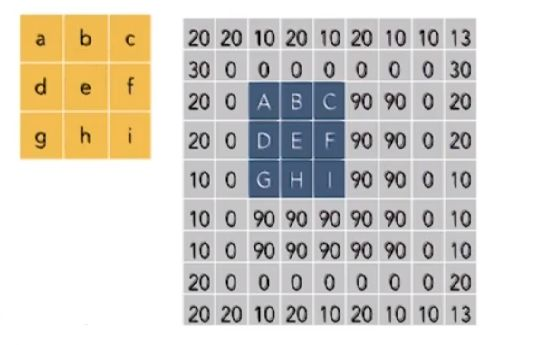
\includegraphics{img/crosscorrelation.jpg}
\caption{title}
\end{figure}

    \[ G[3,3 ] = a*A+b*B+c*C+d*D+e*E+f*F+g*G+h*H+i*I \]

    \paragraph{1.4 Time-series supplemental
materials}\label{time-series-supplemental-materials}

\[ R(i) = \int_{-\infty}^{-\infty}x(t)\cdot y(t+i)dt \]

Where \textbf{x(t)} and \textbf{y(t)} is a function of time;

\begin{verbatim}
 i is the time delay. It can be negative, zero or positive;

 R is corss correlation, which is a function of the time delay i.

 When x(t) = y(t), cross correlation becomes auto correlation.
\end{verbatim}

    \paragraph{1.5 Example}\label{example}

    \[ 1.\ x =[0.1,0.2,-0.1,4.1,-2,1.5,-0.1] \]
\[ 2.\ y =[0.1,4,-2.2,1.6,0.1,0.1,0.2] \]

    \subparagraph{1.5.1 0 time lag}\label{time-lag}

    \begin{Verbatim}[commandchars=\\\{\}]
{\color{incolor}In [{\color{incolor}23}]:} \PY{n}{x} \PY{o}{=} \PY{n}{np}\PY{o}{.}\PY{n}{array}\PY{p}{(}\PY{p}{[}\PY{l+m+mf}{0.1}\PY{p}{,}\PY{l+m+mf}{0.2}\PY{p}{,}\PY{o}{\PYZhy{}}\PY{l+m+mf}{0.1}\PY{p}{,}\PY{l+m+mf}{4.1}\PY{p}{,}\PY{o}{\PYZhy{}}\PY{l+m+mi}{2}\PY{p}{,}\PY{l+m+mf}{1.5}\PY{p}{,}\PY{o}{\PYZhy{}}\PY{l+m+mf}{0.1}\PY{p}{]}\PY{p}{)}
         \PY{n}{y} \PY{o}{=} \PY{n}{np}\PY{o}{.}\PY{n}{array}\PY{p}{(}\PY{p}{[}\PY{l+m+mf}{0.1}\PY{p}{,}\PY{l+m+mi}{4}\PY{p}{,}\PY{o}{\PYZhy{}}\PY{l+m+mf}{2.2}\PY{p}{,}\PY{l+m+mf}{1.6}\PY{p}{,}\PY{l+m+mf}{0.1}\PY{p}{,}\PY{l+m+mf}{0.1}\PY{p}{,}\PY{l+m+mf}{0.2}\PY{p}{]}\PY{p}{)}
         \PY{n}{time} \PY{o}{=} \PY{n}{np}\PY{o}{.}\PY{n}{array}\PY{p}{(}\PY{p}{[}\PY{l+m+mi}{0}\PY{p}{,} \PY{l+m+mi}{1}\PY{p}{,} \PY{l+m+mi}{2}\PY{p}{,} \PY{l+m+mi}{3}\PY{p}{,} \PY{l+m+mi}{4}\PY{p}{,} \PY{l+m+mi}{5}\PY{p}{,} \PY{l+m+mi}{6}\PY{p}{]}\PY{p}{)}
         
         \PY{n}{fig} \PY{o}{=} \PY{n}{plt}\PY{o}{.}\PY{n}{figure}\PY{p}{(}\PY{p}{)}
         
         \PY{n}{ax1} \PY{o}{=} \PY{n}{fig}\PY{o}{.}\PY{n}{add\PYZus{}axes}\PY{p}{(}\PY{p}{[}\PY{l+m+mf}{2.0}\PY{p}{,} \PY{l+m+mf}{1.0}\PY{p}{,} \PY{l+m+mf}{0.8}\PY{p}{,} \PY{l+m+mf}{0.4}\PY{p}{]}\PY{p}{,} \PY{n}{xticklabels}\PY{o}{=}\PY{p}{[}\PY{p}{]}\PY{p}{,} \PY{n}{ylim}\PY{o}{=}\PY{p}{(}\PY{o}{\PYZhy{}}\PY{l+m+mi}{5}\PY{p}{,} \PY{l+m+mi}{5}\PY{p}{)}\PY{p}{)}
         \PY{n}{ax2} \PY{o}{=} \PY{n}{fig}\PY{o}{.}\PY{n}{add\PYZus{}axes}\PY{p}{(}\PY{p}{[}\PY{l+m+mf}{2.0}\PY{p}{,} \PY{l+m+mf}{0.6}\PY{p}{,} \PY{l+m+mf}{0.8}\PY{p}{,} \PY{l+m+mf}{0.4}\PY{p}{]}\PY{p}{,} \PY{n}{ylim}\PY{o}{=}\PY{p}{(}\PY{o}{\PYZhy{}}\PY{l+m+mi}{5}\PY{p}{,} \PY{l+m+mi}{5}\PY{p}{)}\PY{p}{)}
         \PY{n}{ax1}\PY{o}{.}\PY{n}{plot}\PY{p}{(}\PY{n}{time}\PY{p}{,} \PY{n}{x}\PY{p}{,}\PY{l+s+s1}{\PYZsq{}}\PY{l+s+s1}{\PYZhy{}ok}\PY{l+s+s1}{\PYZsq{}}\PY{p}{,} \PY{n}{color}\PY{o}{=}\PY{l+s+s1}{\PYZsq{}}\PY{l+s+s1}{blue}\PY{l+s+s1}{\PYZsq{}}\PY{p}{)}
         \PY{n}{ax2}\PY{o}{.}\PY{n}{plot}\PY{p}{(}\PY{n}{time}\PY{p}{,} \PY{n}{y}\PY{p}{,} \PY{l+s+s1}{\PYZsq{}}\PY{l+s+s1}{\PYZhy{}ok}\PY{l+s+s1}{\PYZsq{}}\PY{p}{,}\PY{n}{color} \PY{o}{=}\PY{l+s+s1}{\PYZsq{}}\PY{l+s+s1}{red}\PY{l+s+s1}{\PYZsq{}}\PY{p}{)}\PY{p}{;}
\end{Verbatim}


    \begin{center}
    \adjustimage{max size={0.9\linewidth}{0.9\paperheight}}{output_26_0.png}
    \end{center}
    { \hspace*{\fill} \\}
    
    \[ Correlation_{zero \ lag} = (0.1)\cdot (0.1)+(0.2)\cdot(0.4)+(-0.1)\cdot(-2.2)+(4.1)\cdot(1.6)+(-2)\cdot(0.1)+(1.5)\cdot(0.1)+(-0.1)\cdot(0.2) =7.52 \]

    \subparagraph{1.5.2 1 time lag}\label{time-lag}

    \begin{Verbatim}[commandchars=\\\{\}]
{\color{incolor}In [{\color{incolor}34}]:} \PY{n}{x} \PY{o}{=} \PY{n}{np}\PY{o}{.}\PY{n}{array}\PY{p}{(}\PY{p}{[}\PY{l+m+mf}{0.1}\PY{p}{,}\PY{l+m+mf}{0.2}\PY{p}{,}\PY{o}{\PYZhy{}}\PY{l+m+mf}{0.1}\PY{p}{,}\PY{l+m+mf}{4.1}\PY{p}{,}\PY{o}{\PYZhy{}}\PY{l+m+mi}{2}\PY{p}{,}\PY{l+m+mf}{1.5}\PY{p}{,}\PY{o}{\PYZhy{}}\PY{l+m+mf}{0.1}\PY{p}{]}\PY{p}{)}
         \PY{n}{y} \PY{o}{=} \PY{n}{np}\PY{o}{.}\PY{n}{array}\PY{p}{(}\PY{p}{[}\PY{l+m+mf}{0.1}\PY{p}{,}\PY{l+m+mi}{4}\PY{p}{,}\PY{o}{\PYZhy{}}\PY{l+m+mf}{2.2}\PY{p}{,}\PY{l+m+mf}{1.6}\PY{p}{,}\PY{l+m+mf}{0.1}\PY{p}{,}\PY{l+m+mf}{0.1}\PY{p}{,}\PY{l+m+mf}{0.2}\PY{p}{]}\PY{p}{)}
         \PY{n}{time} \PY{o}{=} \PY{n}{np}\PY{o}{.}\PY{n}{array}\PY{p}{(}\PY{p}{[}\PY{l+m+mi}{0}\PY{p}{,} \PY{l+m+mi}{1}\PY{p}{,} \PY{l+m+mi}{2}\PY{p}{,} \PY{l+m+mi}{3}\PY{p}{,} \PY{l+m+mi}{4}\PY{p}{,} \PY{l+m+mi}{5}\PY{p}{,} \PY{l+m+mi}{6}\PY{p}{]}\PY{p}{)}
         \PY{n}{fig} \PY{o}{=} \PY{n}{plt}\PY{o}{.}\PY{n}{figure}\PY{p}{(}\PY{p}{)}
         \PY{n}{ax1} \PY{o}{=} \PY{n}{fig}\PY{o}{.}\PY{n}{add\PYZus{}axes}\PY{p}{(}\PY{p}{[}\PY{l+m+mf}{2.0}\PY{p}{,} \PY{l+m+mf}{1.0}\PY{p}{,} \PY{l+m+mf}{0.8}\PY{p}{,} \PY{l+m+mf}{0.4}\PY{p}{]}\PY{p}{,} \PY{n}{xticklabels}\PY{o}{=}\PY{p}{[}\PY{p}{]}\PY{p}{,} \PY{n}{ylim}\PY{o}{=}\PY{p}{(}\PY{o}{\PYZhy{}}\PY{l+m+mi}{5}\PY{p}{,} \PY{l+m+mi}{5}\PY{p}{)}\PY{p}{,} \PY{n}{xlim} \PY{o}{=}\PY{p}{(}\PY{o}{\PYZhy{}}\PY{l+m+mi}{1}\PY{p}{,}\PY{l+m+mi}{8}\PY{p}{)}\PY{p}{)}
         \PY{n}{ax2} \PY{o}{=} \PY{n}{fig}\PY{o}{.}\PY{n}{add\PYZus{}axes}\PY{p}{(}\PY{p}{[}\PY{l+m+mf}{2.0}\PY{p}{,} \PY{l+m+mf}{0.6}\PY{p}{,} \PY{l+m+mf}{0.8}\PY{p}{,} \PY{l+m+mf}{0.4}\PY{p}{]}\PY{p}{,} \PY{n}{ylim}\PY{o}{=}\PY{p}{(}\PY{o}{\PYZhy{}}\PY{l+m+mi}{5}\PY{p}{,} \PY{l+m+mi}{5}\PY{p}{)}\PY{p}{,} \PY{n}{xlim} \PY{o}{=}\PY{p}{(}\PY{o}{\PYZhy{}}\PY{l+m+mi}{1}\PY{p}{,}\PY{l+m+mi}{8}\PY{p}{)}\PY{p}{)}
         \PY{n}{ax1}\PY{o}{.}\PY{n}{plot}\PY{p}{(}\PY{n}{time}\PY{p}{,} \PY{n}{x}\PY{p}{,}\PY{l+s+s1}{\PYZsq{}}\PY{l+s+s1}{\PYZhy{}ok}\PY{l+s+s1}{\PYZsq{}}\PY{p}{,} \PY{n}{color}\PY{o}{=}\PY{l+s+s1}{\PYZsq{}}\PY{l+s+s1}{blue}\PY{l+s+s1}{\PYZsq{}}\PY{p}{)}
         \PY{n}{ax2}\PY{o}{.}\PY{n}{plot}\PY{p}{(}\PY{n}{time}\PY{o}{+}\PY{l+m+mi}{1}\PY{p}{,} \PY{n}{y}\PY{p}{,} \PY{l+s+s1}{\PYZsq{}}\PY{l+s+s1}{\PYZhy{}ok}\PY{l+s+s1}{\PYZsq{}}\PY{p}{,}\PY{n}{color} \PY{o}{=}\PY{l+s+s1}{\PYZsq{}}\PY{l+s+s1}{red}\PY{l+s+s1}{\PYZsq{}}\PY{p}{)}\PY{p}{;}
\end{Verbatim}


    \begin{center}
    \adjustimage{max size={0.9\linewidth}{0.9\paperheight}}{output_29_0.png}
    \end{center}
    { \hspace*{\fill} \\}
    
    \[ Correlation_{one \ lag} = (0.2)\cdot (0.1)+(-0.1)\cdot(4)+(4.1)\cdot(-2.2)+(-2)\cdot(1.6)+(1.5)\cdot(0.1)+(-0.1)\cdot(0.1) =-12.46 \]

    \subparagraph{1.5.3 2 time lag}\label{time-lag}

    \begin{Verbatim}[commandchars=\\\{\}]
{\color{incolor}In [{\color{incolor}35}]:} \PY{n}{x} \PY{o}{=} \PY{n}{np}\PY{o}{.}\PY{n}{array}\PY{p}{(}\PY{p}{[}\PY{l+m+mf}{0.1}\PY{p}{,}\PY{l+m+mf}{0.2}\PY{p}{,}\PY{o}{\PYZhy{}}\PY{l+m+mf}{0.1}\PY{p}{,}\PY{l+m+mf}{4.1}\PY{p}{,}\PY{o}{\PYZhy{}}\PY{l+m+mi}{2}\PY{p}{,}\PY{l+m+mf}{1.5}\PY{p}{,}\PY{o}{\PYZhy{}}\PY{l+m+mf}{0.1}\PY{p}{]}\PY{p}{)}
         \PY{n}{y} \PY{o}{=} \PY{n}{np}\PY{o}{.}\PY{n}{array}\PY{p}{(}\PY{p}{[}\PY{l+m+mf}{0.1}\PY{p}{,}\PY{l+m+mi}{4}\PY{p}{,}\PY{o}{\PYZhy{}}\PY{l+m+mf}{2.2}\PY{p}{,}\PY{l+m+mf}{1.6}\PY{p}{,}\PY{l+m+mf}{0.1}\PY{p}{,}\PY{l+m+mf}{0.1}\PY{p}{,}\PY{l+m+mf}{0.2}\PY{p}{]}\PY{p}{)}
         \PY{n}{time} \PY{o}{=} \PY{n}{np}\PY{o}{.}\PY{n}{array}\PY{p}{(}\PY{p}{[}\PY{l+m+mi}{0}\PY{p}{,} \PY{l+m+mi}{1}\PY{p}{,} \PY{l+m+mi}{2}\PY{p}{,} \PY{l+m+mi}{3}\PY{p}{,} \PY{l+m+mi}{4}\PY{p}{,} \PY{l+m+mi}{5}\PY{p}{,} \PY{l+m+mi}{6}\PY{p}{]}\PY{p}{)}
         \PY{n}{fig} \PY{o}{=} \PY{n}{plt}\PY{o}{.}\PY{n}{figure}\PY{p}{(}\PY{p}{)}
         \PY{n}{ax1} \PY{o}{=} \PY{n}{fig}\PY{o}{.}\PY{n}{add\PYZus{}axes}\PY{p}{(}\PY{p}{[}\PY{l+m+mf}{2.0}\PY{p}{,} \PY{l+m+mf}{1.0}\PY{p}{,} \PY{l+m+mf}{0.8}\PY{p}{,} \PY{l+m+mf}{0.4}\PY{p}{]}\PY{p}{,} \PY{n}{xticklabels}\PY{o}{=}\PY{p}{[}\PY{p}{]}\PY{p}{,} \PY{n}{ylim}\PY{o}{=}\PY{p}{(}\PY{o}{\PYZhy{}}\PY{l+m+mi}{5}\PY{p}{,} \PY{l+m+mi}{5}\PY{p}{)}\PY{p}{,} \PY{n}{xlim} \PY{o}{=}\PY{p}{(}\PY{o}{\PYZhy{}}\PY{l+m+mi}{1}\PY{p}{,}\PY{l+m+mi}{8}\PY{p}{)}\PY{p}{)}
         \PY{n}{ax2} \PY{o}{=} \PY{n}{fig}\PY{o}{.}\PY{n}{add\PYZus{}axes}\PY{p}{(}\PY{p}{[}\PY{l+m+mf}{2.0}\PY{p}{,} \PY{l+m+mf}{0.6}\PY{p}{,} \PY{l+m+mf}{0.8}\PY{p}{,} \PY{l+m+mf}{0.4}\PY{p}{]}\PY{p}{,} \PY{n}{ylim}\PY{o}{=}\PY{p}{(}\PY{o}{\PYZhy{}}\PY{l+m+mi}{5}\PY{p}{,} \PY{l+m+mi}{5}\PY{p}{)}\PY{p}{,} \PY{n}{xlim} \PY{o}{=}\PY{p}{(}\PY{o}{\PYZhy{}}\PY{l+m+mi}{1}\PY{p}{,}\PY{l+m+mi}{8}\PY{p}{)}\PY{p}{)}
         \PY{n}{ax1}\PY{o}{.}\PY{n}{plot}\PY{p}{(}\PY{n}{time}\PY{p}{,} \PY{n}{x}\PY{p}{,}\PY{l+s+s1}{\PYZsq{}}\PY{l+s+s1}{\PYZhy{}ok}\PY{l+s+s1}{\PYZsq{}}\PY{p}{,} \PY{n}{color}\PY{o}{=}\PY{l+s+s1}{\PYZsq{}}\PY{l+s+s1}{blue}\PY{l+s+s1}{\PYZsq{}}\PY{p}{)}
         \PY{n}{ax2}\PY{o}{.}\PY{n}{plot}\PY{p}{(}\PY{n}{time}\PY{o}{+}\PY{l+m+mi}{2}\PY{p}{,} \PY{n}{y}\PY{p}{,} \PY{l+s+s1}{\PYZsq{}}\PY{l+s+s1}{\PYZhy{}ok}\PY{l+s+s1}{\PYZsq{}}\PY{p}{,}\PY{n}{color} \PY{o}{=}\PY{l+s+s1}{\PYZsq{}}\PY{l+s+s1}{red}\PY{l+s+s1}{\PYZsq{}}\PY{p}{)}\PY{p}{;}
\end{Verbatim}


    \begin{center}
    \adjustimage{max size={0.9\linewidth}{0.9\paperheight}}{output_32_0.png}
    \end{center}
    { \hspace*{\fill} \\}
    
    \[ Correlation_{two \ lag} = (-0.1)\cdot(0.1)+(4.1)\cdot(4)+(-2)\cdot(-2.2)+(1.5)\cdot(1.6)+(-0.1)\cdot(0.1) =23.18 \]

    \subparagraph{1.5.4 Result}\label{result}

    \[ Correlation\_Sequence = [7.52, -12.46, 23.18, -11.05, 6.02, -0.25, -0.01] \]

    \paragraph{1.6 Python Library
Calculation}\label{python-library-calculation}

    \begin{Verbatim}[commandchars=\\\{\}]
{\color{incolor}In [{\color{incolor}48}]:} \PY{n}{x} \PY{o}{=} \PY{n}{np}\PY{o}{.}\PY{n}{array}\PY{p}{(}\PY{p}{[}\PY{l+m+mf}{0.1}\PY{p}{,}\PY{l+m+mf}{0.2}\PY{p}{,}\PY{o}{\PYZhy{}}\PY{l+m+mf}{0.1}\PY{p}{,}\PY{l+m+mf}{4.1}\PY{p}{,}\PY{o}{\PYZhy{}}\PY{l+m+mi}{2}\PY{p}{,}\PY{l+m+mf}{1.5}\PY{p}{,}\PY{o}{\PYZhy{}}\PY{l+m+mf}{0.1}\PY{p}{]}\PY{p}{)}
         \PY{n}{y} \PY{o}{=} \PY{n}{np}\PY{o}{.}\PY{n}{array}\PY{p}{(}\PY{p}{[}\PY{l+m+mf}{0.1}\PY{p}{,}\PY{l+m+mi}{4}\PY{p}{,}\PY{o}{\PYZhy{}}\PY{l+m+mf}{2.2}\PY{p}{,}\PY{l+m+mf}{1.6}\PY{p}{,}\PY{l+m+mf}{0.1}\PY{p}{,}\PY{l+m+mf}{0.1}\PY{p}{,}\PY{l+m+mf}{0.2}\PY{p}{]}\PY{p}{)}
         \PY{n}{np}\PY{o}{.}\PY{n}{correlate}\PY{p}{(}\PY{n}{x}\PY{p}{,} \PY{n}{y}\PY{p}{,} \PY{l+s+s2}{\PYZdq{}}\PY{l+s+s2}{same}\PY{l+s+s2}{\PYZdq{}}\PY{p}{)}
\end{Verbatim}


\begin{Verbatim}[commandchars=\\\{\}]
{\color{outcolor}Out[{\color{outcolor}48}]:} array([  0.99,   0.1 ,   0.31,   7.52, -12.46,  23.18, -11.05])
\end{Verbatim}
            
    \begin{Verbatim}[commandchars=\\\{\}]
{\color{incolor}In [{\color{incolor}115}]:} \PY{k+kn}{from} \PY{n+nn}{scipy} \PY{k}{import} \PY{n}{signal}
          \PY{n}{x} \PY{o}{=} \PY{n}{np}\PY{o}{.}\PY{n}{array}\PY{p}{(}\PY{p}{[}\PY{l+m+mf}{0.1}\PY{p}{,}\PY{l+m+mf}{0.2}\PY{p}{,}\PY{o}{\PYZhy{}}\PY{l+m+mf}{0.1}\PY{p}{,}\PY{l+m+mf}{4.1}\PY{p}{,}\PY{o}{\PYZhy{}}\PY{l+m+mi}{2}\PY{p}{,}\PY{l+m+mf}{1.5}\PY{p}{,}\PY{o}{\PYZhy{}}\PY{l+m+mf}{0.1}\PY{p}{]}\PY{p}{)}
          \PY{n}{y} \PY{o}{=} \PY{n}{np}\PY{o}{.}\PY{n}{array}\PY{p}{(}\PY{p}{[}\PY{l+m+mf}{0.1}\PY{p}{,}\PY{l+m+mi}{4}\PY{p}{,}\PY{o}{\PYZhy{}}\PY{l+m+mf}{2.2}\PY{p}{,}\PY{l+m+mf}{1.6}\PY{p}{,}\PY{l+m+mf}{0.1}\PY{p}{,}\PY{l+m+mf}{0.1}\PY{p}{,}\PY{l+m+mf}{0.2}\PY{p}{]}\PY{p}{)}
          \PY{n}{corr} \PY{o}{=} \PY{n}{signal}\PY{o}{.}\PY{n}{correlate}\PY{p}{(}\PY{n}{x}\PY{p}{,} \PY{n}{y}\PY{p}{,} \PY{n}{mode} \PY{o}{=}\PY{l+s+s1}{\PYZsq{}}\PY{l+s+s1}{same}\PY{l+s+s1}{\PYZsq{}}\PY{p}{)}
          \PY{n}{corr}
\end{Verbatim}


\begin{Verbatim}[commandchars=\\\{\}]
{\color{outcolor}Out[{\color{outcolor}115}]:} array([  0.99,   0.1 ,   0.31,   7.52, -12.46,  23.18, -11.05])
\end{Verbatim}
            
    \begin{Verbatim}[commandchars=\\\{\}]
{\color{incolor}In [{\color{incolor}118}]:} \PY{n}{fig} \PY{o}{=} \PY{n}{plt}\PY{o}{.}\PY{n}{figure}\PY{p}{(}\PY{p}{)}
          \PY{c+c1}{\PYZsh{} Search trend volume}
          \PY{n}{ax1} \PY{o}{=} \PY{n}{fig}\PY{o}{.}\PY{n}{add\PYZus{}subplot}\PY{p}{(}\PY{l+m+mi}{311}\PY{p}{)}
          \PY{n}{ax1}\PY{o}{.}\PY{n}{plot}\PY{p}{(}\PY{n}{x}\PY{p}{)}
          \PY{n}{ax1}\PY{o}{.}\PY{n}{set\PYZus{}xlabel}\PY{p}{(}\PY{l+s+s1}{\PYZsq{}}\PY{l+s+s1}{x data}\PY{l+s+s1}{\PYZsq{}}\PY{p}{)}
          
          \PY{n}{total} \PY{o}{=} \PY{n+nb}{sum}\PY{p}{(}\PY{n}{x}\PY{p}{)}
          \PY{n}{av} \PY{o}{=} \PY{n}{total} \PY{o}{/} \PY{n+nb}{len}\PY{p}{(}\PY{n}{x}\PY{p}{)}
          \PY{n}{z} \PY{o}{=} \PY{p}{[}\PY{n}{i} \PY{o}{\PYZhy{}} \PY{n}{av} \PY{k}{for} \PY{n}{i} \PY{o+ow}{in} \PY{n}{x}\PY{p}{]}
          
          \PY{c+c1}{\PYZsh{} Random: \PYZdq{}search trend volume\PYZdq{}}
          \PY{n}{ax2} \PY{o}{=} \PY{n}{fig}\PY{o}{.}\PY{n}{add\PYZus{}subplot}\PY{p}{(}\PY{l+m+mi}{312}\PY{p}{)}
          \PY{n}{ax2}\PY{o}{.}\PY{n}{plot}\PY{p}{(}\PY{n}{y}\PY{p}{)}
          \PY{n}{ax2}\PY{o}{.}\PY{n}{set\PYZus{}xlabel}\PY{p}{(}\PY{l+s+s1}{\PYZsq{}}\PY{l+s+s1}{y data}\PY{l+s+s1}{\PYZsq{}}\PY{p}{)}
          
          \PY{n}{total1} \PY{o}{=} \PY{n+nb}{sum}\PY{p}{(}\PY{n}{y}\PY{p}{)}
          \PY{n}{av1} \PY{o}{=} \PY{n}{total1} \PY{o}{/} \PY{n+nb}{len}\PY{p}{(}\PY{n}{y}\PY{p}{)}
          \PY{n}{z1} \PY{o}{=} \PY{p}{[}\PY{n}{i} \PY{o}{\PYZhy{}} \PY{n}{av1} \PY{k}{for} \PY{n}{i} \PY{o+ow}{in} \PY{n}{y}\PY{p}{]}
          
          \PY{c+c1}{\PYZsh{} Is there a pattern in search trend for this keyword?}
          \PY{n}{ax3} \PY{o}{=} \PY{n}{fig}\PY{o}{.}\PY{n}{add\PYZus{}subplot}\PY{p}{(}\PY{l+m+mi}{313}\PY{p}{)}
          \PY{n}{ax3}\PY{o}{.}\PY{n}{set\PYZus{}xlabel}\PY{p}{(}\PY{l+s+s1}{\PYZsq{}}\PY{l+s+s1}{Cross correlation of random data}\PY{l+s+s1}{\PYZsq{}}\PY{p}{)}
          \PY{n}{ax3}\PY{o}{.}\PY{n}{xcorr}\PY{p}{(}\PY{n}{z}\PY{p}{,} \PY{n}{z1}\PY{p}{,} \PY{n}{usevlines}\PY{o}{=}\PY{k+kc}{True}\PY{p}{,} \PY{n}{maxlags}\PY{o}{=}\PY{k+kc}{None}\PY{p}{,} \PY{n}{normed}\PY{o}{=}\PY{k+kc}{False}\PY{p}{,} \PY{n}{lw}\PY{o}{=}\PY{l+m+mi}{2}\PY{p}{)}
          \PY{n}{ax3}\PY{o}{.}\PY{n}{grid}\PY{p}{(}\PY{k+kc}{True}\PY{p}{)}
          \PY{n}{plt}\PY{o}{.}\PY{n}{ylim}\PY{p}{(}\PY{o}{\PYZhy{}}\PY{l+m+mi}{15}\PY{p}{,} \PY{l+m+mi}{25}\PY{p}{)}
          \PY{n}{plt}\PY{o}{.}\PY{n}{tight\PYZus{}layout}\PY{p}{(}\PY{p}{)}
          \PY{n}{plt}\PY{o}{.}\PY{n}{show}\PY{p}{(}\PY{p}{)}\PY{p}{;}
\end{Verbatim}


    \begin{center}
    \adjustimage{max size={0.9\linewidth}{0.9\paperheight}}{output_39_0.png}
    \end{center}
    { \hspace*{\fill} \\}
    
    \subsection{2 Normalized
cross-correlation}\label{normalized-cross-correlation}

The \textbf{comparison} of \textbf{two time series}, but using \textbf{a
different scoring result}. Instead of simple cross-correlation, it can
compare metrics with \textbf{different value ranges}.

    \[ NCC =\frac{\sum_{i=1}^{MN}x_{i}y_{i}}{\sqrt{\sum_{i=1}^{MN}x_{i}^{2}\cdot\sum_{i=1}^{MN}y_{i}^{2} }} \]

    \paragraph{2.1 Example}\label{example}

    \begin{Verbatim}[commandchars=\\\{\}]
{\color{incolor}In [{\color{incolor}119}]:} \PY{n}{x} \PY{o}{=} \PY{n}{np}\PY{o}{.}\PY{n}{array}\PY{p}{(}\PY{p}{[}\PY{l+m+mf}{1.0}\PY{p}{,}\PY{l+m+mf}{2.0}\PY{p}{,}\PY{l+m+mf}{3.0}\PY{p}{]}\PY{p}{)}
          \PY{n}{y} \PY{o}{=} \PY{n}{np}\PY{o}{.}\PY{n}{array}\PY{p}{(}\PY{p}{[}\PY{l+m+mf}{1.0}\PY{p}{,}\PY{l+m+mf}{2.0}\PY{p}{,}\PY{l+m+mf}{3.0}\PY{p}{]}\PY{p}{)}
          \PY{k+kn}{from} \PY{n+nn}{obspy}\PY{n+nn}{.}\PY{n+nn}{signal}\PY{n+nn}{.}\PY{n+nn}{cross\PYZus{}correlation} \PY{k}{import} \PY{n}{correlate}
          \PY{n}{correlate}\PY{p}{(}\PY{n}{x}\PY{p}{,}\PY{n}{y}\PY{p}{,}\PY{n}{shift}\PY{o}{=}\PY{l+m+mi}{2}\PY{p}{,}\PY{n}{normalize}\PY{o}{=}\PY{k+kc}{True}\PY{p}{,} \PY{n}{demean}\PY{o}{=}\PY{k+kc}{False}\PY{p}{)}
\end{Verbatim}


\begin{Verbatim}[commandchars=\\\{\}]
{\color{outcolor}Out[{\color{outcolor}119}]:} array([ 0.21428571,  0.57142857,  1.        ,  0.57142857,  0.21428571])
\end{Verbatim}
            
    \begin{Verbatim}[commandchars=\\\{\}]
{\color{incolor}In [{\color{incolor}123}]:} \PY{n}{x} \PY{o}{=} \PY{n}{np}\PY{o}{.}\PY{n}{array}\PY{p}{(}\PY{p}{[}\PY{l+m+mf}{1.0}\PY{p}{,}\PY{l+m+mf}{2.0}\PY{p}{,}\PY{l+m+mf}{3.0}\PY{p}{]}\PY{p}{)}
          \PY{n}{y} \PY{o}{=} \PY{n}{np}\PY{o}{.}\PY{n}{array}\PY{p}{(}\PY{p}{[}\PY{l+m+mf}{1.0}\PY{p}{,}\PY{l+m+mf}{2.0}\PY{p}{,}\PY{l+m+mf}{3.0}\PY{p}{]}\PY{p}{)}
          \PY{n}{fig} \PY{o}{=} \PY{n}{plt}\PY{o}{.}\PY{n}{figure}\PY{p}{(}\PY{p}{)}
          \PY{n}{ax1} \PY{o}{=} \PY{n}{fig}\PY{o}{.}\PY{n}{add\PYZus{}subplot}\PY{p}{(}\PY{l+m+mi}{111}\PY{p}{)}
          \PY{n}{ax1}\PY{o}{.}\PY{n}{xcorr}\PY{p}{(}\PY{n}{x}\PY{p}{,} \PY{n}{y}\PY{p}{,} \PY{n}{usevlines}\PY{o}{=}\PY{k+kc}{True}\PY{p}{,} \PY{n}{maxlags}\PY{o}{=}\PY{l+m+mi}{2}\PY{p}{,} \PY{n}{normed}\PY{o}{=}\PY{k+kc}{True}\PY{p}{,} \PY{n}{lw}\PY{o}{=}\PY{l+m+mi}{2}\PY{p}{)}
          \PY{n}{ax1}\PY{o}{.}\PY{n}{grid}\PY{p}{(}\PY{k+kc}{True}\PY{p}{)}
          \PY{n}{ax1}\PY{o}{.}\PY{n}{set\PYZus{}ylim}\PY{p}{(}\PY{l+m+mi}{0}\PY{p}{,} \PY{l+m+mf}{1.1}\PY{p}{)}
          \PY{n}{ax1}\PY{o}{.}\PY{n}{axhline}\PY{p}{(}\PY{l+m+mi}{0}\PY{p}{,} \PY{n}{color}\PY{o}{=}\PY{l+s+s1}{\PYZsq{}}\PY{l+s+s1}{black}\PY{l+s+s1}{\PYZsq{}}\PY{p}{,} \PY{n}{lw}\PY{o}{=}\PY{l+m+mi}{2}\PY{p}{)}
          \PY{n}{plt}\PY{o}{.}\PY{n}{show}\PY{p}{(}\PY{p}{)}\PY{p}{;}
\end{Verbatim}


    \begin{center}
    \adjustimage{max size={0.9\linewidth}{0.9\paperheight}}{output_44_0.png}
    \end{center}
    { \hspace*{\fill} \\}
    
    \paragraph{2.2 Zero-mean Normalized
Cross-Correlation}\label{zero-mean-normalized-cross-correlation}

    \[ ZNCC =\frac{\sum_{i=1}^{MN}(x_{i}-\bar{x})(y_{i}-\bar{y})}{\sqrt{\sum_{i=1}^{MN}(x_{i}-\bar{x})^{2}\cdot\sum_{i=1}^{MN}(y_{i}-\bar{y})^{2} }} \]

    where \textbf{x̄} and \textbf{ȳ} are the \textbf{mean intensity values}.

    \begin{Verbatim}[commandchars=\\\{\}]
{\color{incolor}In [{\color{incolor}128}]:} \PY{n}{x} \PY{o}{=} \PY{n}{np}\PY{o}{.}\PY{n}{array}\PY{p}{(}\PY{p}{[}\PY{l+m+mf}{1.0}\PY{p}{,}\PY{l+m+mf}{2.0}\PY{p}{,}\PY{l+m+mf}{3.0}\PY{p}{]}\PY{p}{)}
          \PY{n}{y} \PY{o}{=} \PY{n}{np}\PY{o}{.}\PY{n}{array}\PY{p}{(}\PY{p}{[}\PY{l+m+mf}{1.0}\PY{p}{,}\PY{l+m+mf}{1.0}\PY{p}{,}\PY{l+m+mf}{2.0}\PY{p}{]}\PY{p}{)}
          \PY{k+kn}{from} \PY{n+nn}{obspy}\PY{n+nn}{.}\PY{n+nn}{signal}\PY{n+nn}{.}\PY{n+nn}{cross\PYZus{}correlation} \PY{k}{import} \PY{n}{correlate}
          \PY{n}{result} \PY{o}{=} \PY{n}{correlate}\PY{p}{(}\PY{n}{x}\PY{p}{,}\PY{n}{y}\PY{p}{,}\PY{n}{shift}\PY{o}{=}\PY{l+m+mi}{2}\PY{p}{,}\PY{n}{normalize}\PY{o}{=}\PY{k+kc}{True}\PY{p}{,} \PY{n}{demean}\PY{o}{=}\PY{k+kc}{True}\PY{p}{)}
          \PY{n}{result}
\end{Verbatim}


\begin{Verbatim}[commandchars=\\\{\}]
{\color{outcolor}Out[{\color{outcolor}128}]:} array([-0.57735027,  0.28867513,  0.8660254 , -0.28867513, -0.28867513])
\end{Verbatim}
            
    \begin{Verbatim}[commandchars=\\\{\}]
{\color{incolor}In [{\color{incolor}135}]:} \PY{n}{x} \PY{o}{=} \PY{n}{np}\PY{o}{.}\PY{n}{array}\PY{p}{(}\PY{p}{[}\PY{o}{\PYZhy{}}\PY{l+m+mi}{2}\PY{p}{,}\PY{o}{\PYZhy{}}\PY{l+m+mi}{1}\PY{p}{,}\PY{l+m+mi}{0}\PY{p}{,}\PY{l+m+mi}{1}\PY{p}{,}\PY{l+m+mi}{2}\PY{p}{]}\PY{p}{)}
          \PY{n}{y} \PY{o}{=} \PY{n}{result}
          \PY{n}{fig} \PY{o}{=} \PY{n}{plt}\PY{o}{.}\PY{n}{figure}\PY{p}{(}\PY{p}{)}
          \PY{n}{ax1} \PY{o}{=} \PY{n}{fig}\PY{o}{.}\PY{n}{add\PYZus{}axes}\PY{p}{(}\PY{p}{[}\PY{l+m+mf}{2.0}\PY{p}{,} \PY{l+m+mf}{1.0}\PY{p}{,} \PY{l+m+mf}{0.8}\PY{p}{,} \PY{l+m+mf}{0.4}\PY{p}{]}\PY{p}{,} \PY{n}{xticklabels}\PY{o}{=}\PY{p}{[}\PY{o}{\PYZhy{}}\PY{l+m+mi}{3}\PY{p}{,}\PY{o}{\PYZhy{}}\PY{l+m+mi}{2}\PY{p}{,}\PY{o}{\PYZhy{}}\PY{l+m+mi}{1}\PY{p}{,}\PY{l+m+mi}{0}\PY{p}{,}\PY{l+m+mi}{1}\PY{p}{,}\PY{l+m+mi}{2}\PY{p}{,}\PY{l+m+mi}{3}\PY{p}{]}\PY{p}{,} \PY{n}{ylim}\PY{o}{=}\PY{p}{(}\PY{o}{\PYZhy{}}\PY{l+m+mi}{1}\PY{p}{,} \PY{l+m+mi}{1}\PY{p}{)}\PY{p}{,} \PY{n}{xlim} \PY{o}{=}\PY{p}{(}\PY{o}{\PYZhy{}}\PY{l+m+mi}{3}\PY{p}{,}\PY{l+m+mi}{3}\PY{p}{)}\PY{p}{)}
          \PY{n}{ax1}\PY{o}{.}\PY{n}{plot}\PY{p}{(}\PY{n}{x}\PY{p}{,} \PY{n}{y}\PY{p}{,} \PY{l+s+s1}{\PYZsq{}}\PY{l+s+s1}{\PYZhy{}ok}\PY{l+s+s1}{\PYZsq{}}\PY{p}{,}\PY{n}{color} \PY{o}{=}\PY{l+s+s1}{\PYZsq{}}\PY{l+s+s1}{red}\PY{l+s+s1}{\PYZsq{}}\PY{p}{)}\PY{p}{;}
\end{Verbatim}


    \begin{center}
    \adjustimage{max size={0.9\linewidth}{0.9\paperheight}}{output_49_0.png}
    \end{center}
    { \hspace*{\fill} \\}
    
    \paragraph{2.3 Auto-correlation}\label{auto-correlation}

    The \textbf{comparison} of a \textbf{time series} with itself at a
\textbf{different time}. It aims, for example, to \textbf{detect
repeating patterns or seasonality}. For example: ``Is there weekly
seasonality on a server website?'' ``Does the current week's data highly
correlate with that of the previous week?''

You can see the example from \textbf{Normalized cross-correlation}.

\href{https://docs.scipy.org/doc/scipy-0.18.1/reference/generated/scipy.signal.correlate.html}{scipy.signal.correlate}

    \subsection{3. Convolution}\label{convolution}

    \paragraph{3.1 Formula}\label{formula}

    \[ G[i,j]=\sum_{v=-k}^{k}\sum_{v=-k}^{k}h[u,v]\cdot F[i-u,j-v] \]
Denoted by: \[ G = h*F \]

\href{https://zh.wikipedia.org/wiki/\%E5\%8D\%B7\%E7\%A7\%AF}{Convolution}

\href{https://currents.soest.hawaii.edu/ocn_data_analysis/_static/SEM_EDOF.html}{ocn\_data\_analysis}

\href{https://currents.soest.hawaii.edu/ocn_data_analysis/_static/SEM_EDOF.html}{relate
material}

    \textbf{Flip fliter} in both dimensions

\begin{verbatim}
1) Bottom to Top
2) Right to Left
\end{verbatim}

Then apply \textbf{cross-correlation}

    \begin{figure}
\centering
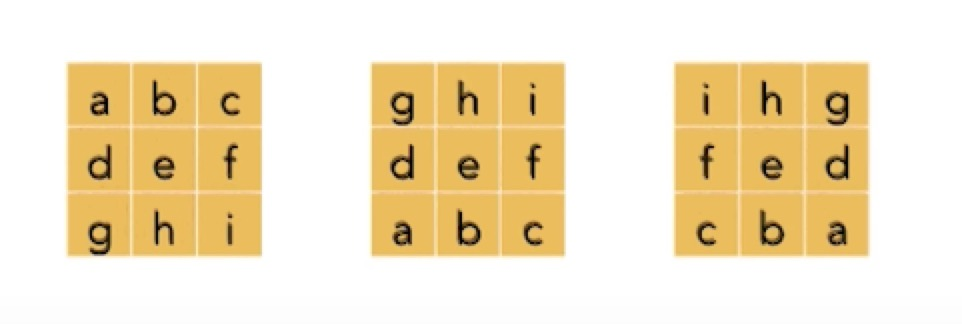
\includegraphics{img/convolution.jpg}
\caption{title}
\end{figure}

    \paragraph{3.2 1-D Formula}\label{d-formula}

    \[ y(t)=\int_{-\infty}^{+\infty}x(\imath )h(t-\imath )d\imath = \int_{-\infty}^{+\infty}h(\imath )x(t-\imath )d\imath \]

    \paragraph{3.3 Cross-correlation vs
Convolution}\label{cross-correlation-vs-convolution}

    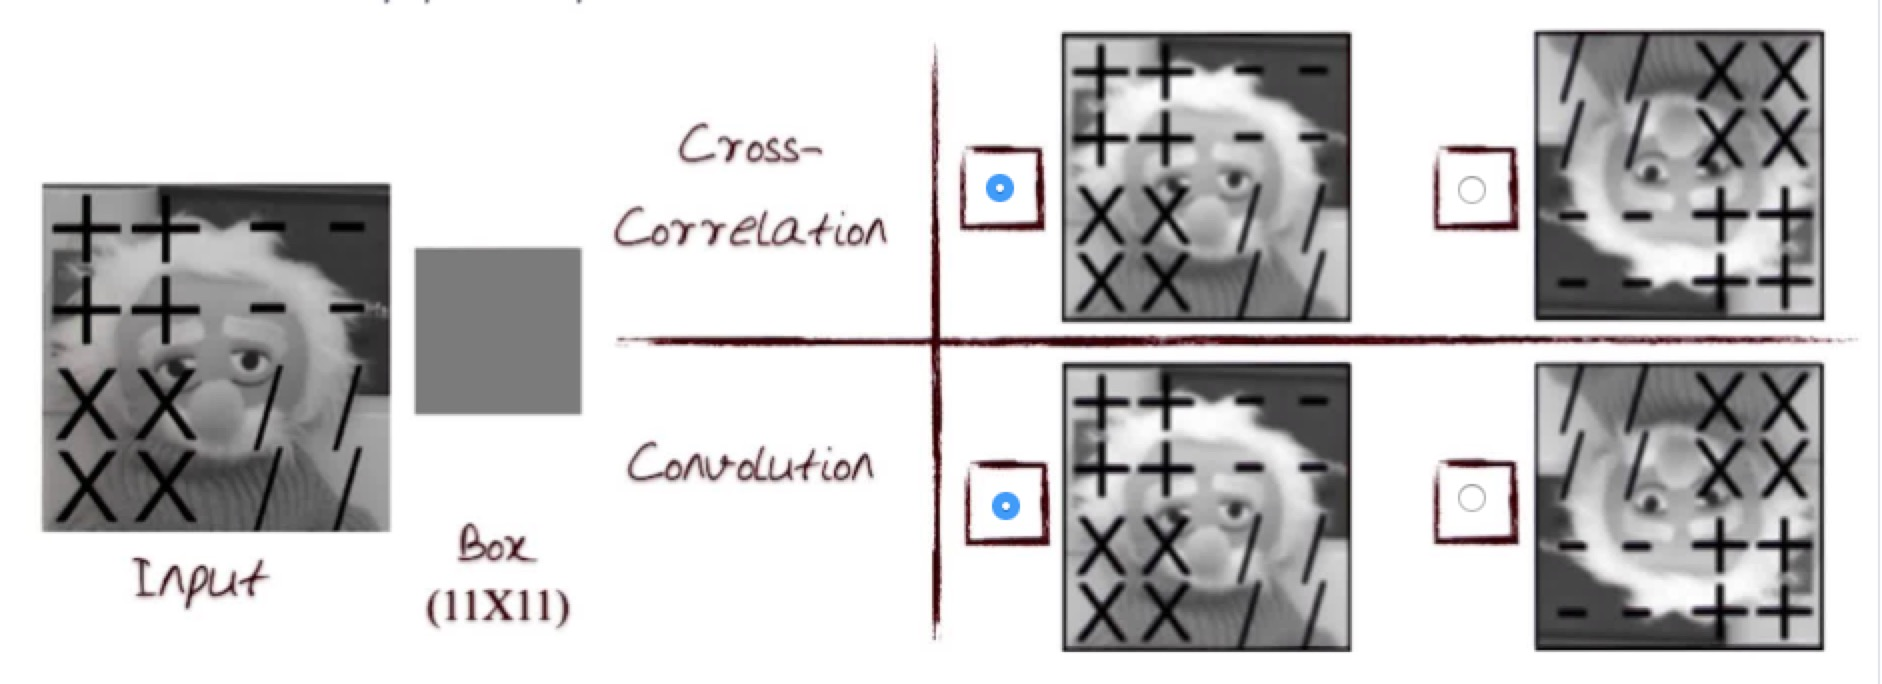
\includegraphics{img/compare_1.jpg} 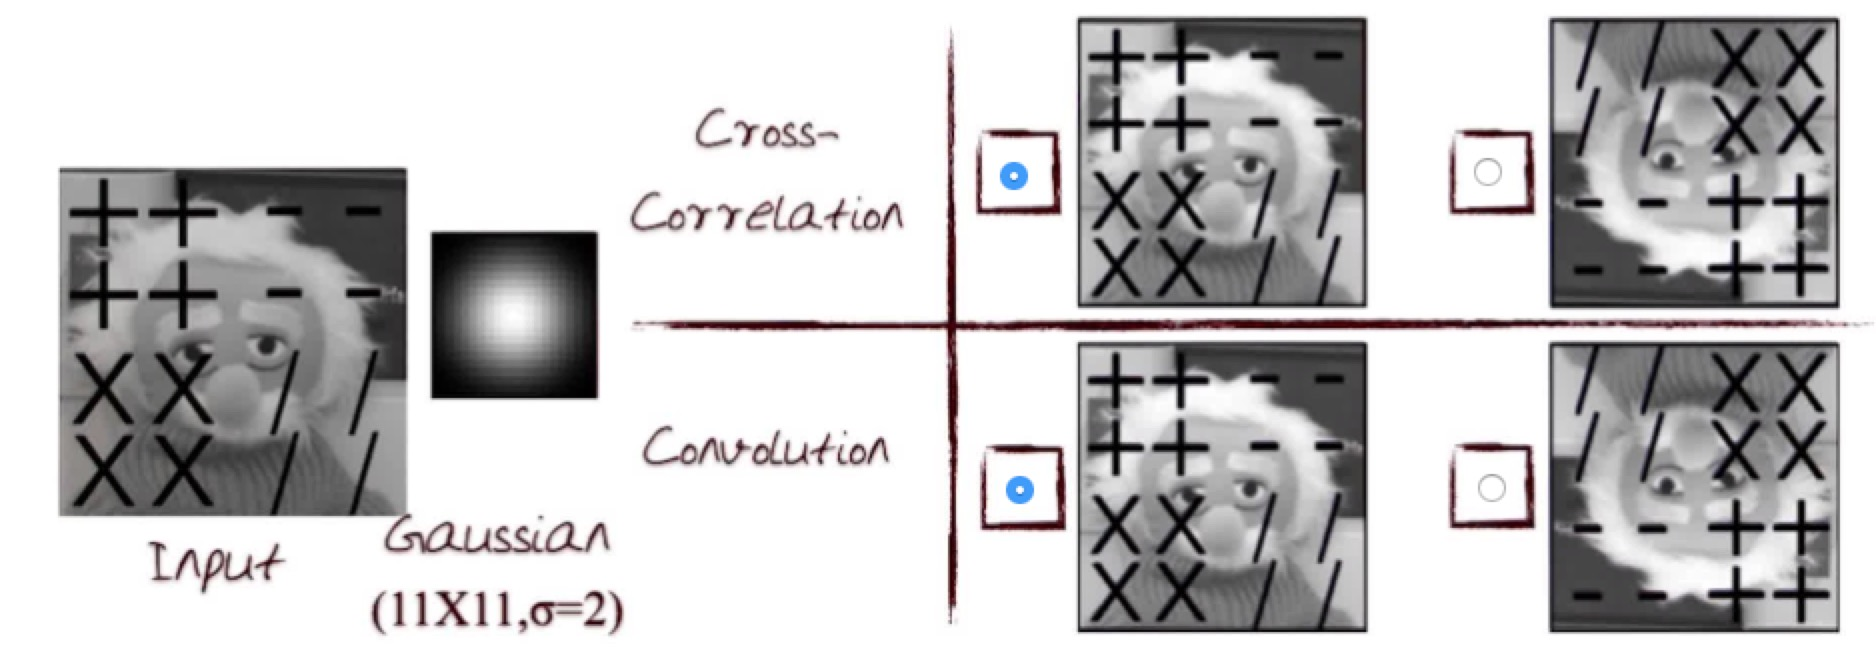
\includegraphics{img/compare_2.jpg}
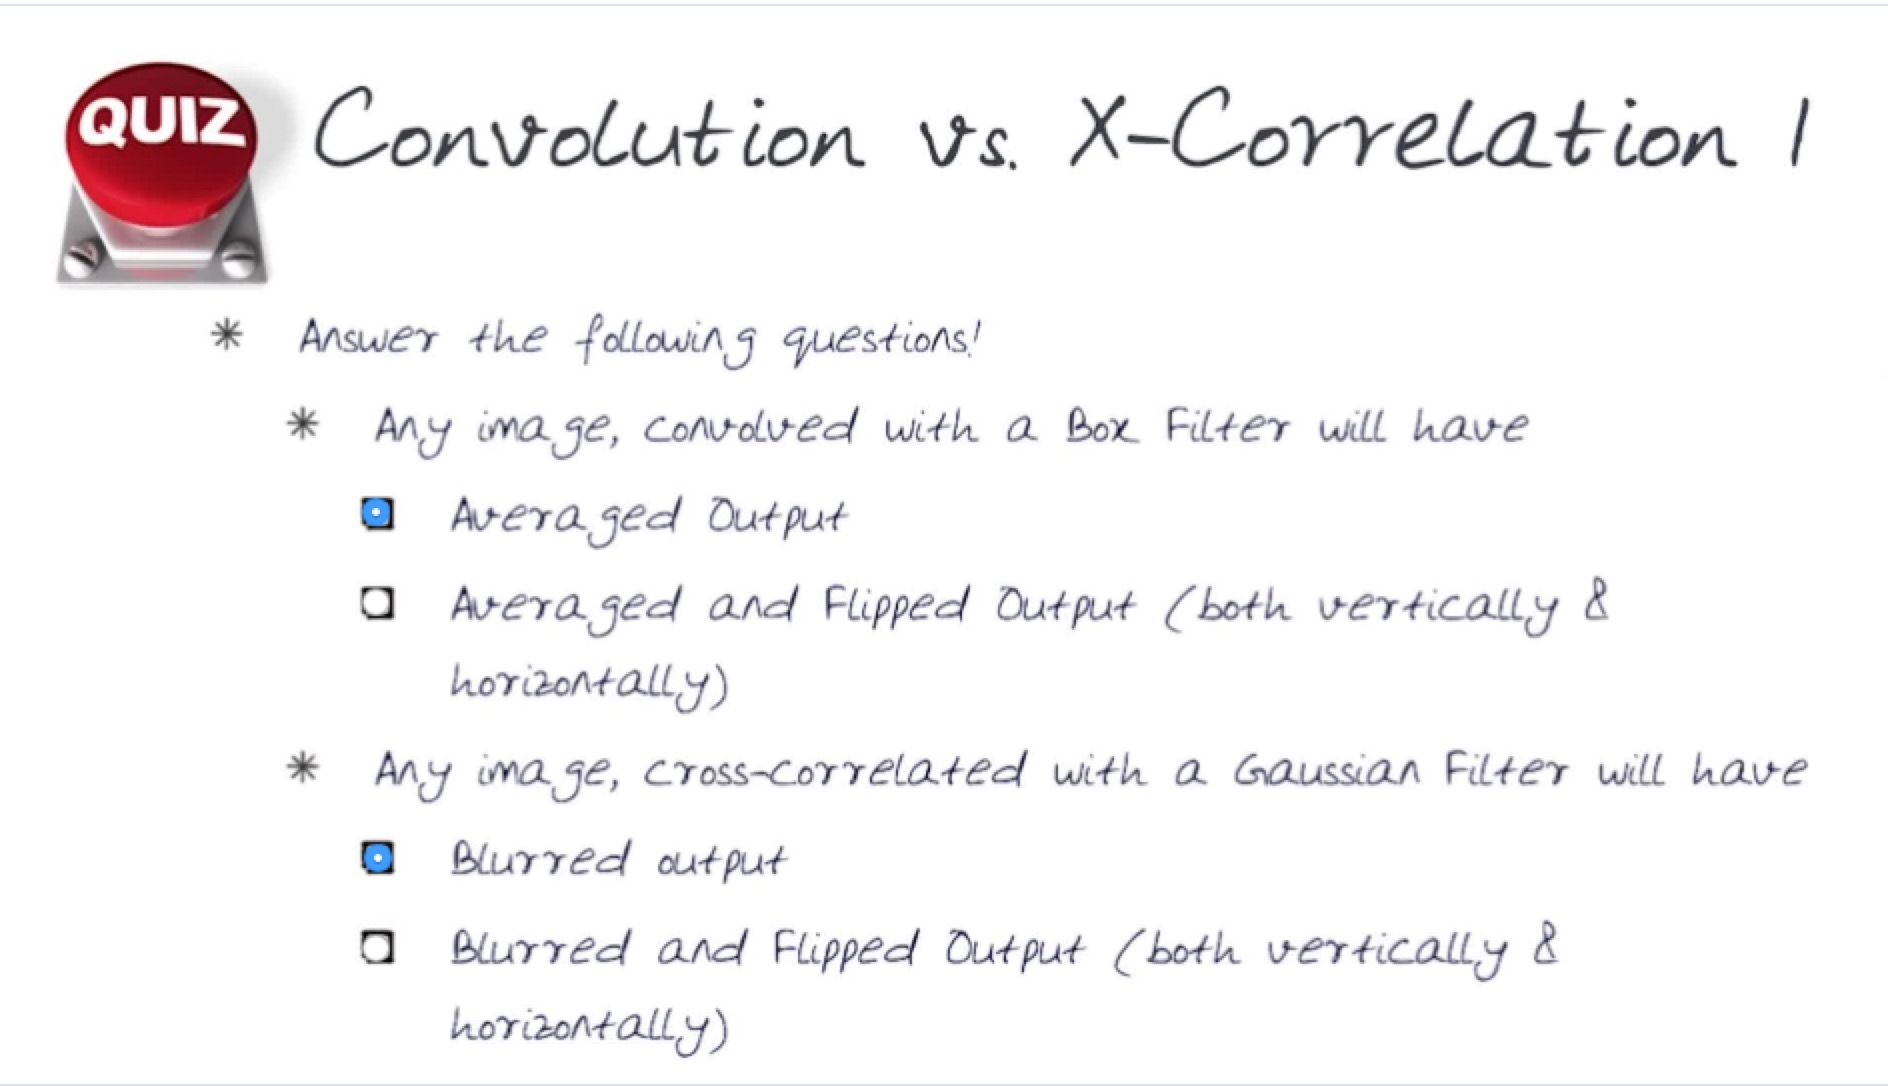
\includegraphics{img/compare_3.jpg} 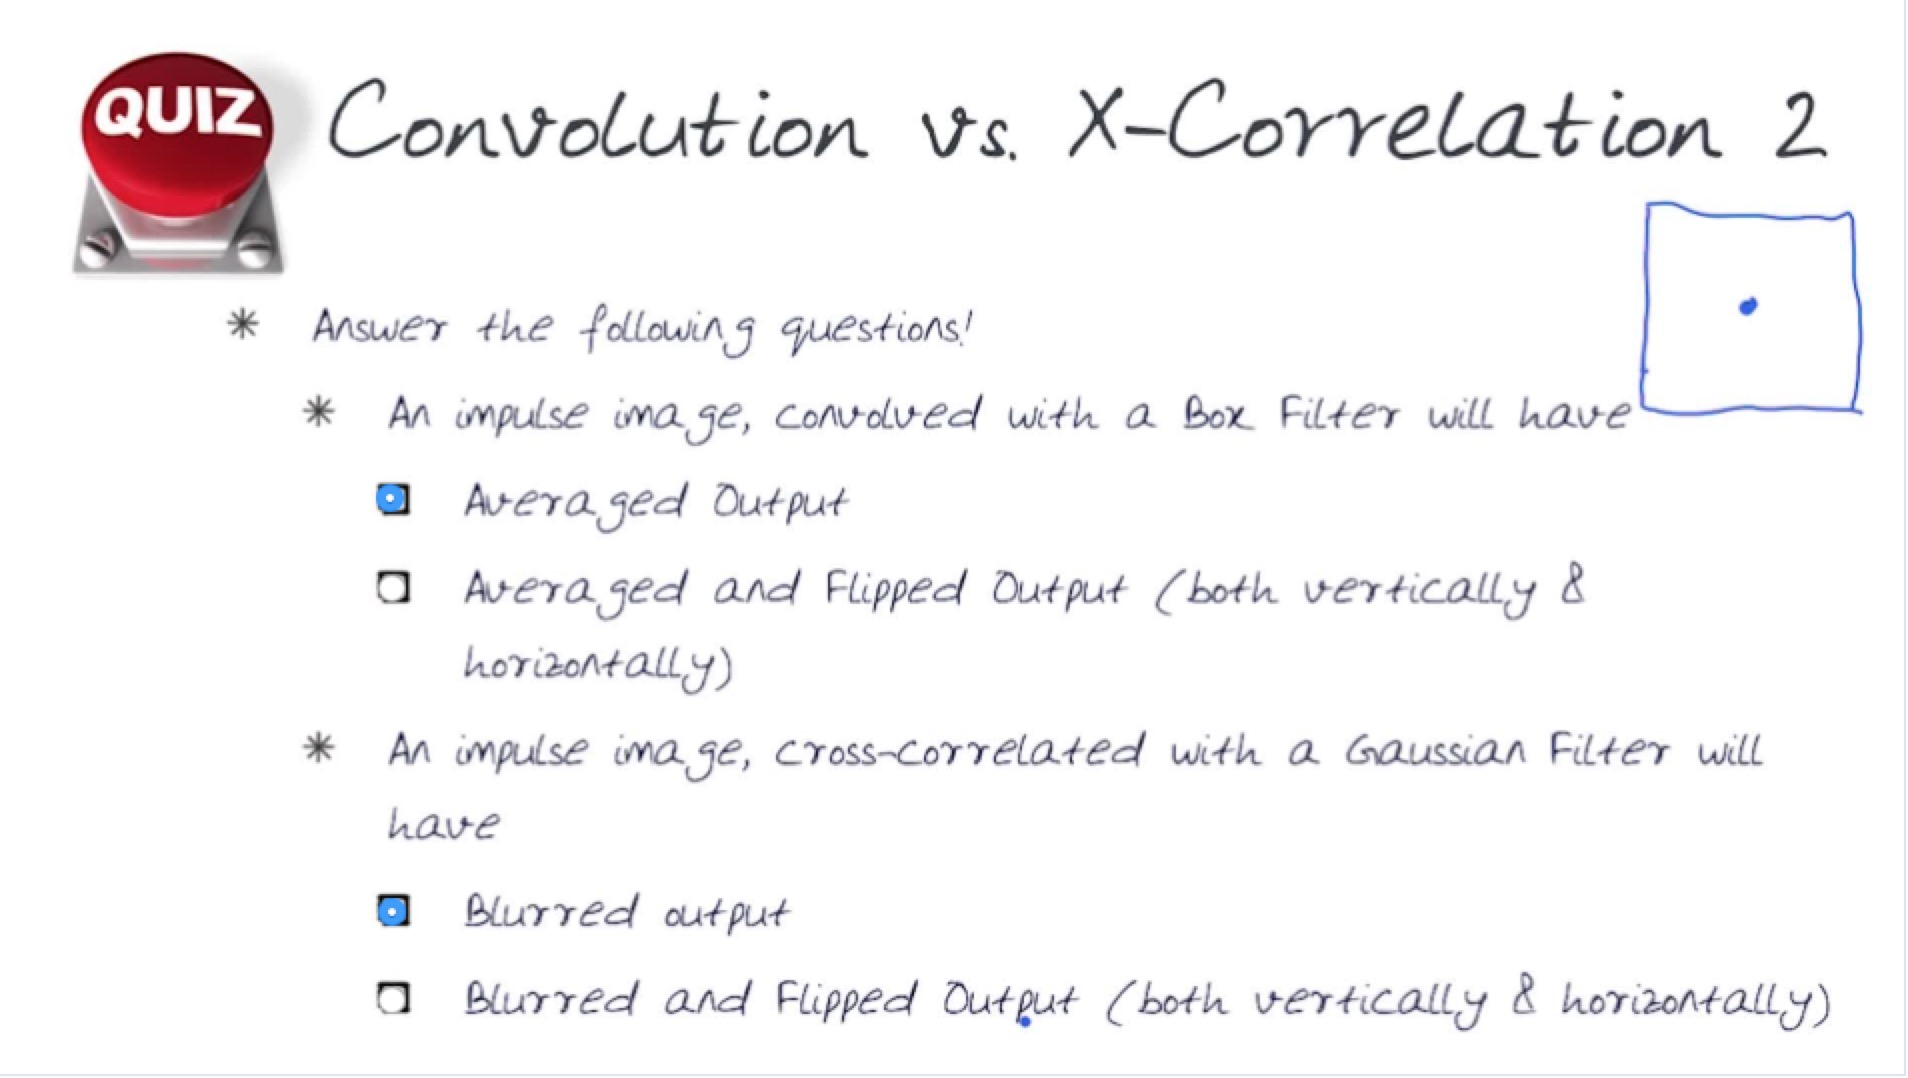
\includegraphics{img/compare_4.jpg}
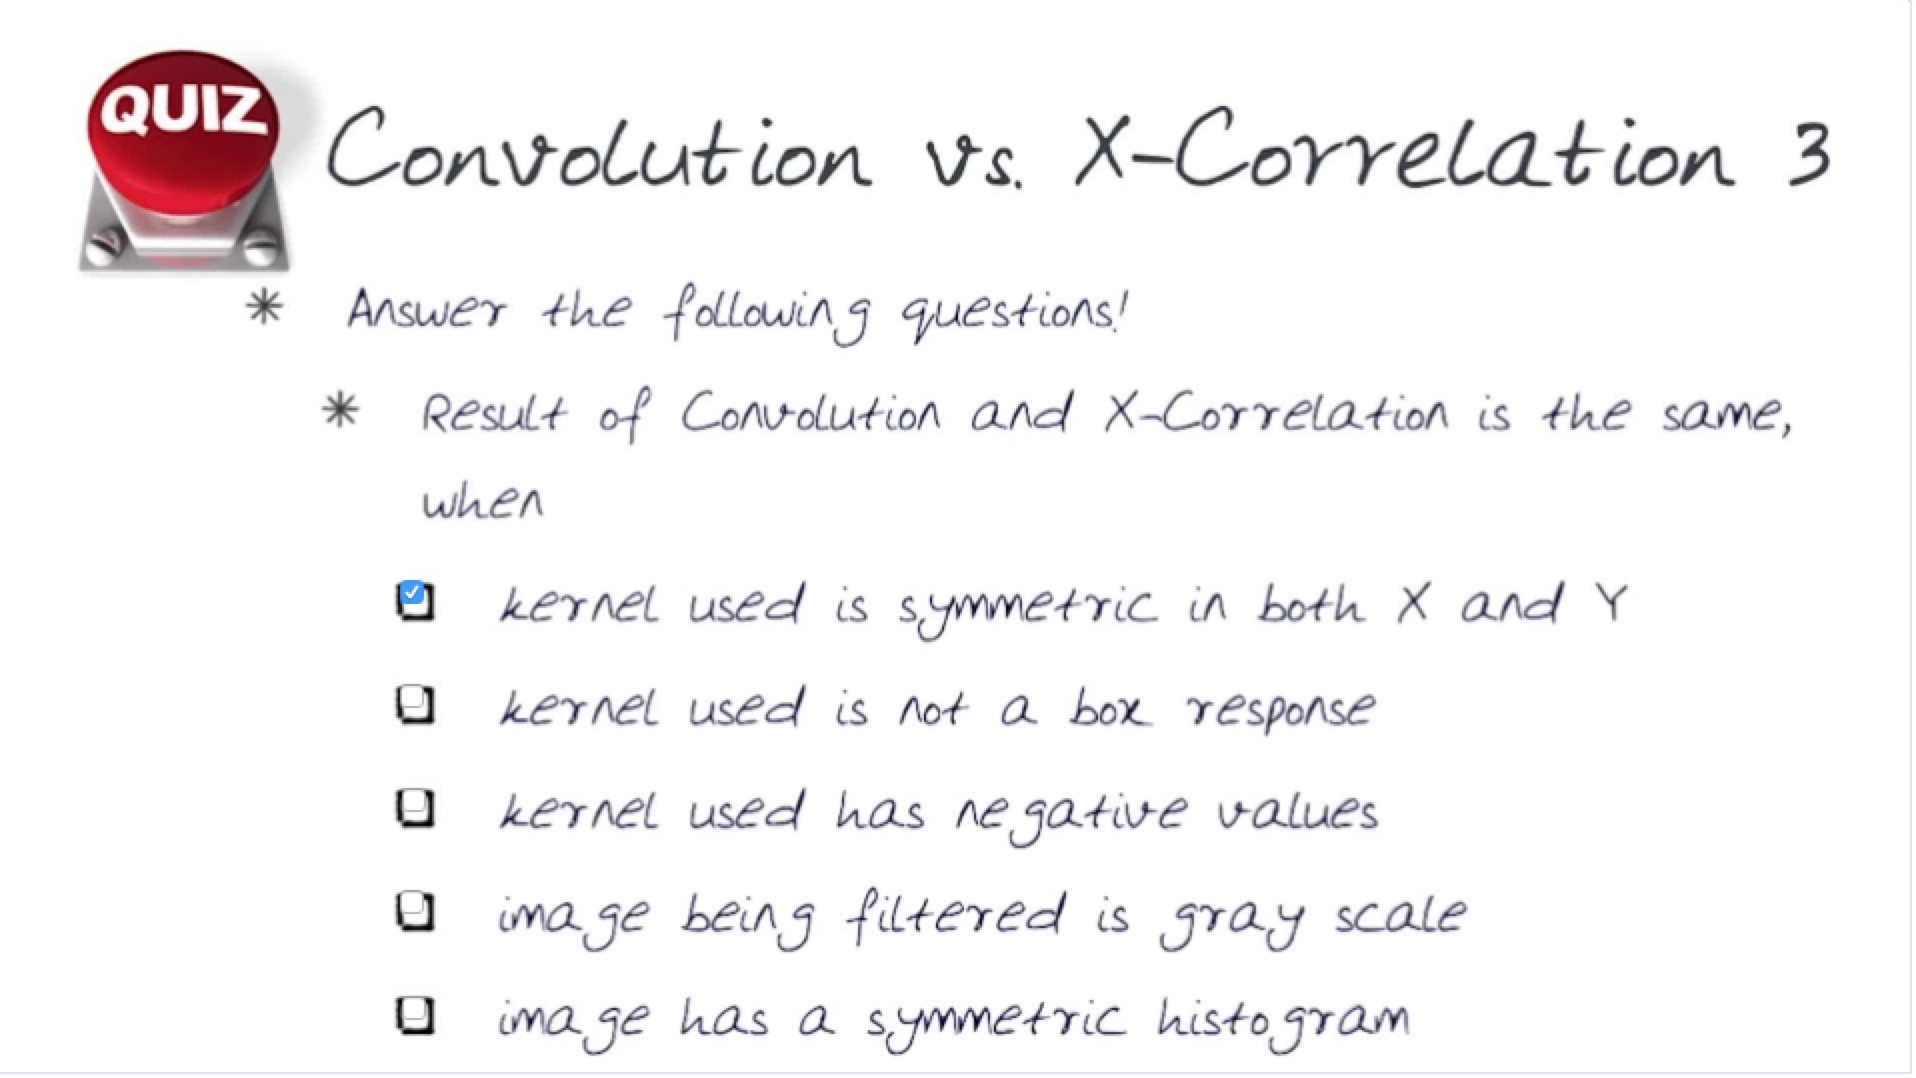
\includegraphics{img/compare_5.jpg} 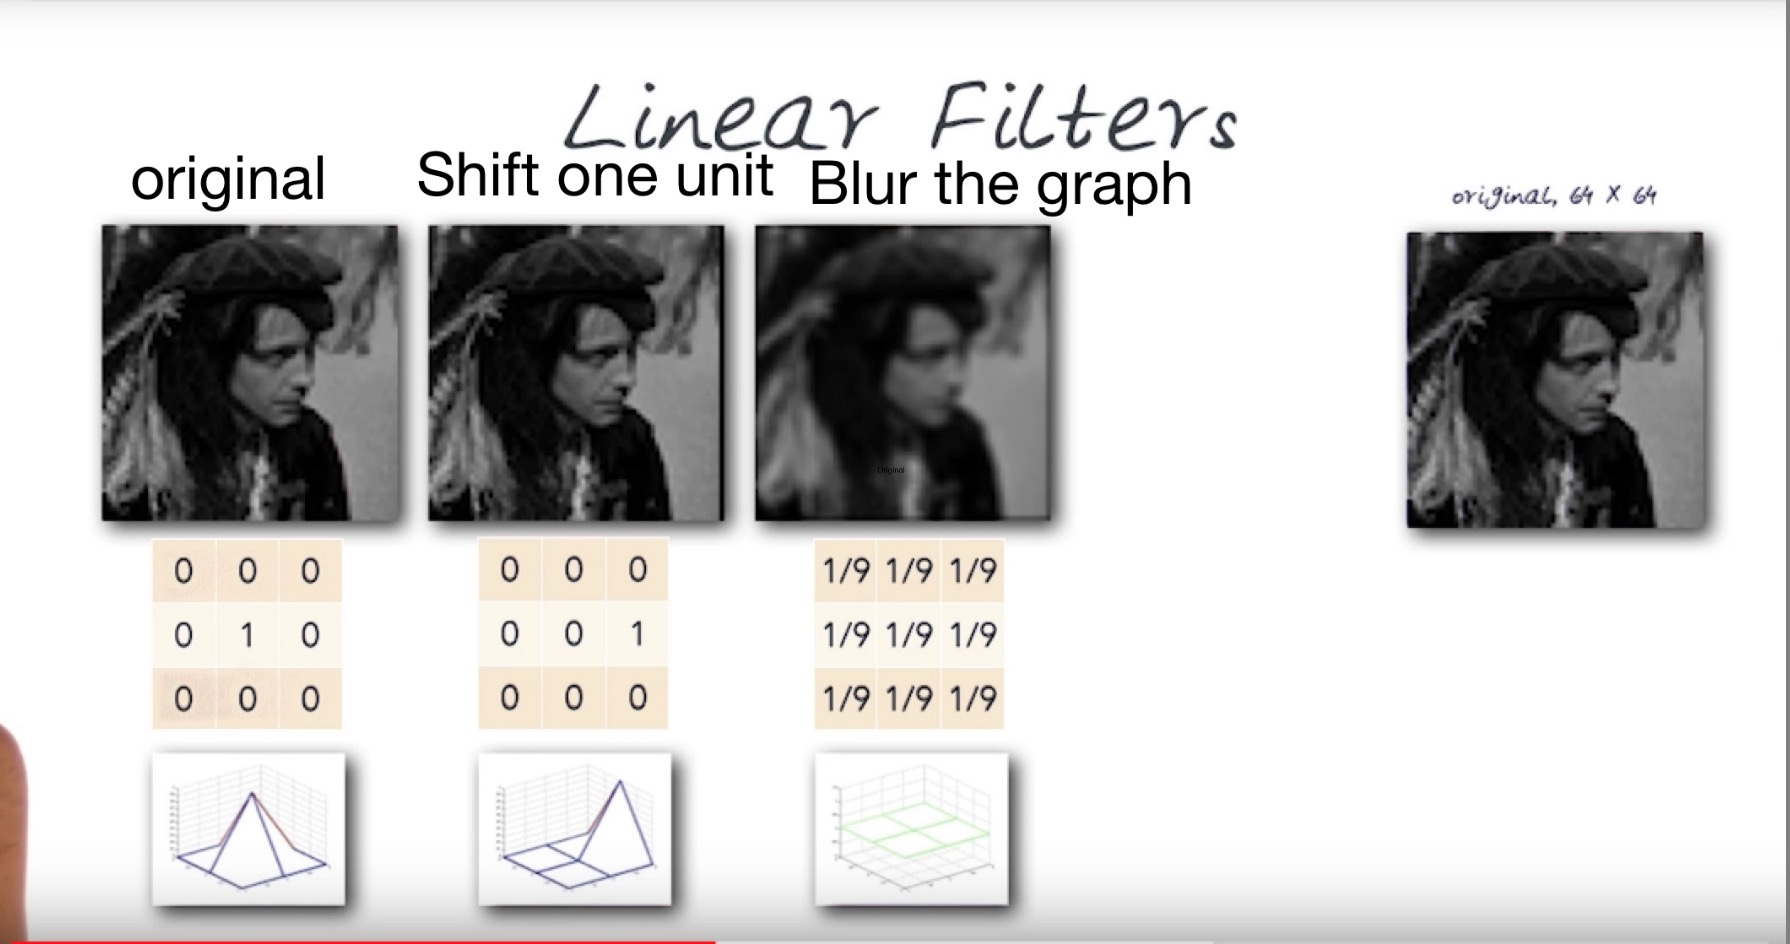
\includegraphics{img/compare_6.jpg}
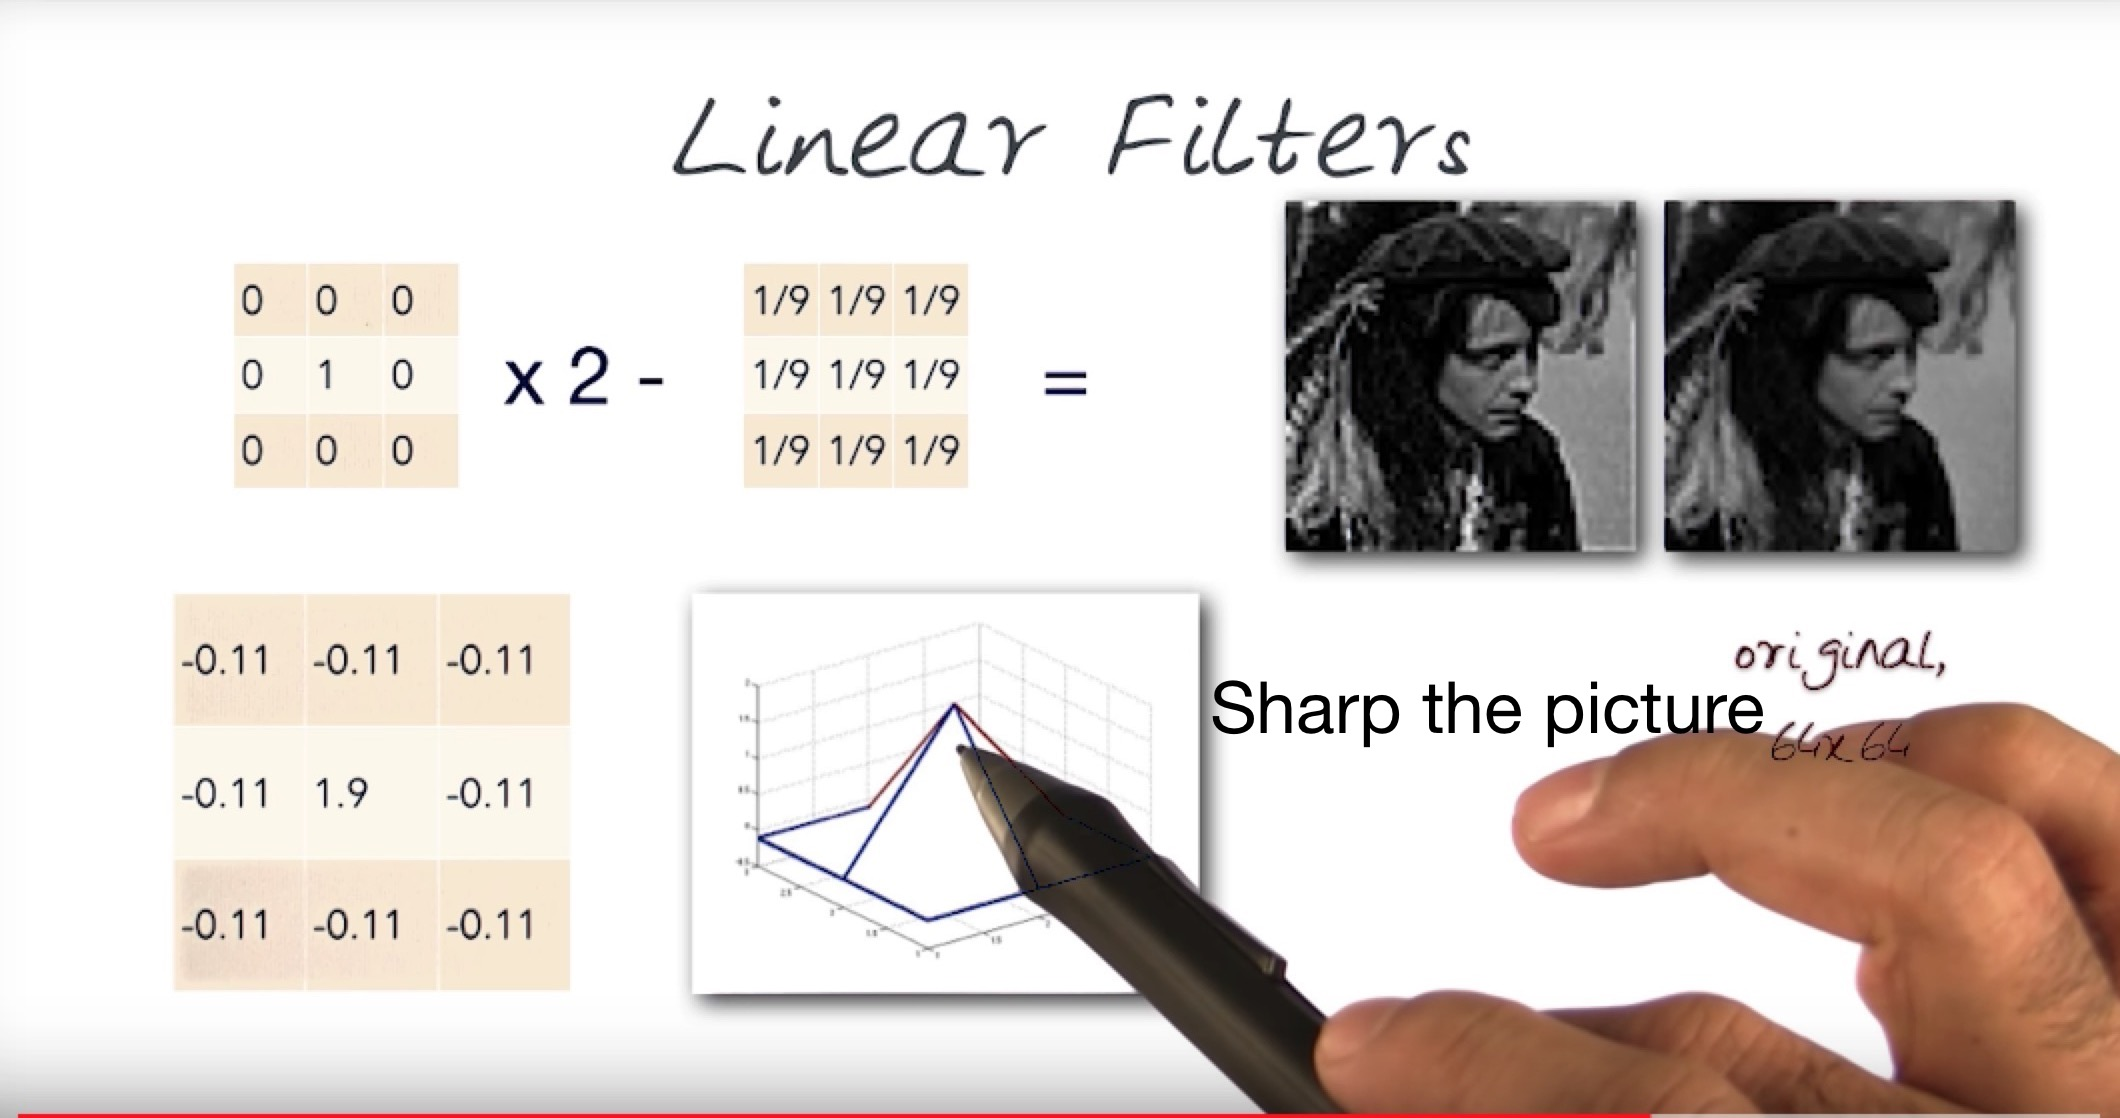
\includegraphics{img/compare_7.jpg}

    \paragraph{3.4 Properties of
Convolution}\label{properties-of-convolution}

    \begin{enumerate}
\def\labelenumi{\arabic{enumi})}
\item
  Linear and Shift Invariants

  Behaves the same everywhere(i.e., the value of the output depends on
  the pattern in the image neighborhood, not the position of the
  neigborhood)
\item
  Commutative \[ F*G=G*F \]
\item
  Associative \[ (F*G)*H=F*(G*H) \]
\item
  Identity: Unit Impulse E={[}....0, 0, 1, 0, 0,....{]},

  F*E=F
\item
  Separable If the filter is separable, convolve all rows, then convolve
  all columns
\end{enumerate}

    \paragraph{3.5 Demo Code}\label{demo-code}

    \begin{Verbatim}[commandchars=\\\{\}]
{\color{incolor}In [{\color{incolor}137}]:} \PY{c+c1}{\PYZsh{} Note how the convolution operator flips the second array before “sliding” the two across one another:}
          \PY{n+nb}{print}\PY{p}{(}\PY{n}{np}\PY{o}{.}\PY{n}{convolve}\PY{p}{(}\PY{p}{[}\PY{l+m+mi}{1}\PY{p}{,} \PY{l+m+mi}{2}\PY{p}{,} \PY{l+m+mi}{3}\PY{p}{]}\PY{p}{,} \PY{p}{[}\PY{l+m+mi}{0}\PY{p}{,} \PY{l+m+mi}{1}\PY{p}{,} \PY{l+m+mf}{0.5}\PY{p}{]}\PY{p}{)}\PY{p}{)}
          
          \PY{c+c1}{\PYZsh{} Only return the middle values of the convolution. Contains boundary effects, where zeros are taken into account:}
          \PY{n+nb}{print}\PY{p}{(}\PY{n}{np}\PY{o}{.}\PY{n}{convolve}\PY{p}{(}\PY{p}{[}\PY{l+m+mi}{1}\PY{p}{,}\PY{l+m+mi}{2}\PY{p}{,}\PY{l+m+mi}{3}\PY{p}{]}\PY{p}{,}\PY{p}{[}\PY{l+m+mi}{0}\PY{p}{,}\PY{l+m+mi}{1}\PY{p}{,}\PY{l+m+mf}{0.5}\PY{p}{]}\PY{p}{,} \PY{l+s+s1}{\PYZsq{}}\PY{l+s+s1}{same}\PY{l+s+s1}{\PYZsq{}}\PY{p}{)}\PY{p}{)}
          
          \PY{c+c1}{\PYZsh{} The two arrays are of the same length, so there is only one position where they completely overlap:}
          \PY{n+nb}{print}\PY{p}{(}\PY{n}{np}\PY{o}{.}\PY{n}{convolve}\PY{p}{(}\PY{p}{[}\PY{l+m+mi}{1}\PY{p}{,}\PY{l+m+mi}{2}\PY{p}{,}\PY{l+m+mi}{3}\PY{p}{]}\PY{p}{,}\PY{p}{[}\PY{l+m+mi}{0}\PY{p}{,}\PY{l+m+mi}{1}\PY{p}{,}\PY{l+m+mf}{0.5}\PY{p}{]}\PY{p}{,} \PY{l+s+s1}{\PYZsq{}}\PY{l+s+s1}{valid}\PY{l+s+s1}{\PYZsq{}}\PY{p}{)}\PY{p}{)}
\end{Verbatim}


    \begin{Verbatim}[commandchars=\\\{\}]
[ 0.   1.   2.5  4.   1.5]
[ 1.   2.5  4. ]
[ 2.5]

    \end{Verbatim}


    % Add a bibliography block to the postdoc
    
    
    
    \end{document}
